\documentclass[../notes.tex]{subfiles}

\pagestyle{main}
\renewcommand{\chaptermark}[1]{\markboth{\chaptername\ \thechapter\ (#1)}{}}
\setcounter{chapter}{4}

\begin{document}




\chapter{Enolate Chemistry}
\setcounter{section}{28}
\section{Enols and Enolates}
\begin{itemize}
    \item \marginnote{11/15:}Grade cutoffs on Exam 3.
    \begin{itemize}
        \item A: 85-100.
        \item B: 70-84.
        \item C: 63-69.
        \item $<\text{C}$: $<57$.
        \item If you are considering dropping this class, the drop date is 11/20.
        \begin{itemize}
            \item It does not count as a drop if you just stop showing up and stop submitting assignments.
            \item Go to the Registrar's site and fill out an add/drop form.
        \end{itemize}
        \item If you are doing less well than you had hoped or expected, talk to your TFs about options!
        \begin{itemize}
            \item You may be eligible for tutoring.
            \item It is \emph{your responsibility} to reach out for help.
        \end{itemize}
    \end{itemize}
    \item Fun (or scary) Friday: Prof. Buchwald sings the elements song!
    \item Announcement: Unit 5 study guide posted.
    \item We now begin the first of four lectures in Unit 5: Enols and enolates.
    \begin{itemize}
        \item Readings: Chapters 20, 25, 26 of \textcite{bib:Clayden}.
    \end{itemize}
    \item Lecture outline.
    \begin{enumerate}[label={\Alph*.}]
        \item Background.
        \begin{itemize}
            \item Enolate definition.
            \item Keto-enol tautomerization (base-catalyzed and acid-catalyzed).
            \item Evidence: Deuterium exchange.
        \end{itemize}
        \item $\alpha$-halogenation of ketones.
        \begin{itemize}
            \item Base-promoted mechanism (and complications).
            \item The iodoform reaction.
            \item Acid-catalyzed mechanism.
        \end{itemize}
        \item $\alpha$-alkylation.
        \begin{itemize}
            % \item General form.
            \item Lithium diisopropylamide.
            \item Malonate ester synthesis.
            \item Kinetic vs. thermodynamic enolates.
        \end{itemize}
    \end{enumerate}
    \pagebreak
    \item We'll begin with Topic A: Background.
    \item Defining enolates.
    \begin{figure}[h!]
        \centering
        \begin{subfigure}[b]{0.4\linewidth}
            \centering
            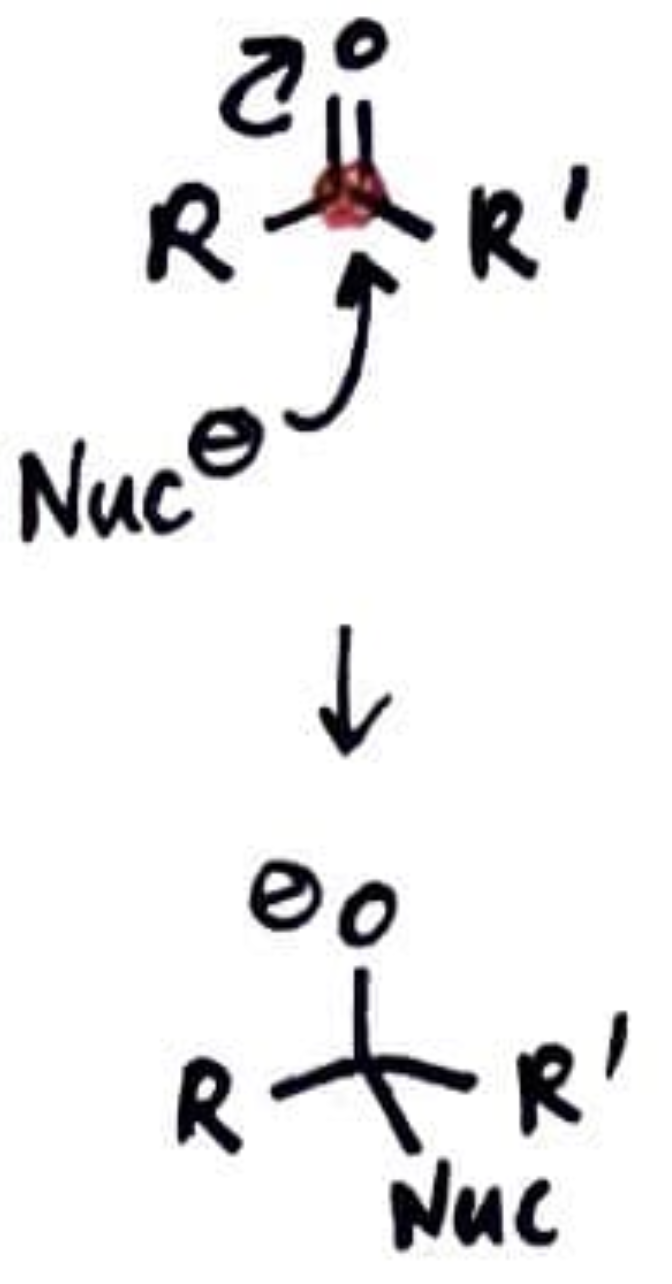
\includegraphics[width=0.23\linewidth]{carbonylRxna.png}
            \caption{As electrophile.}
            \label{fig:carbonylRxna}
        \end{subfigure}
        \begin{subfigure}[b]{0.4\linewidth}
            \centering
            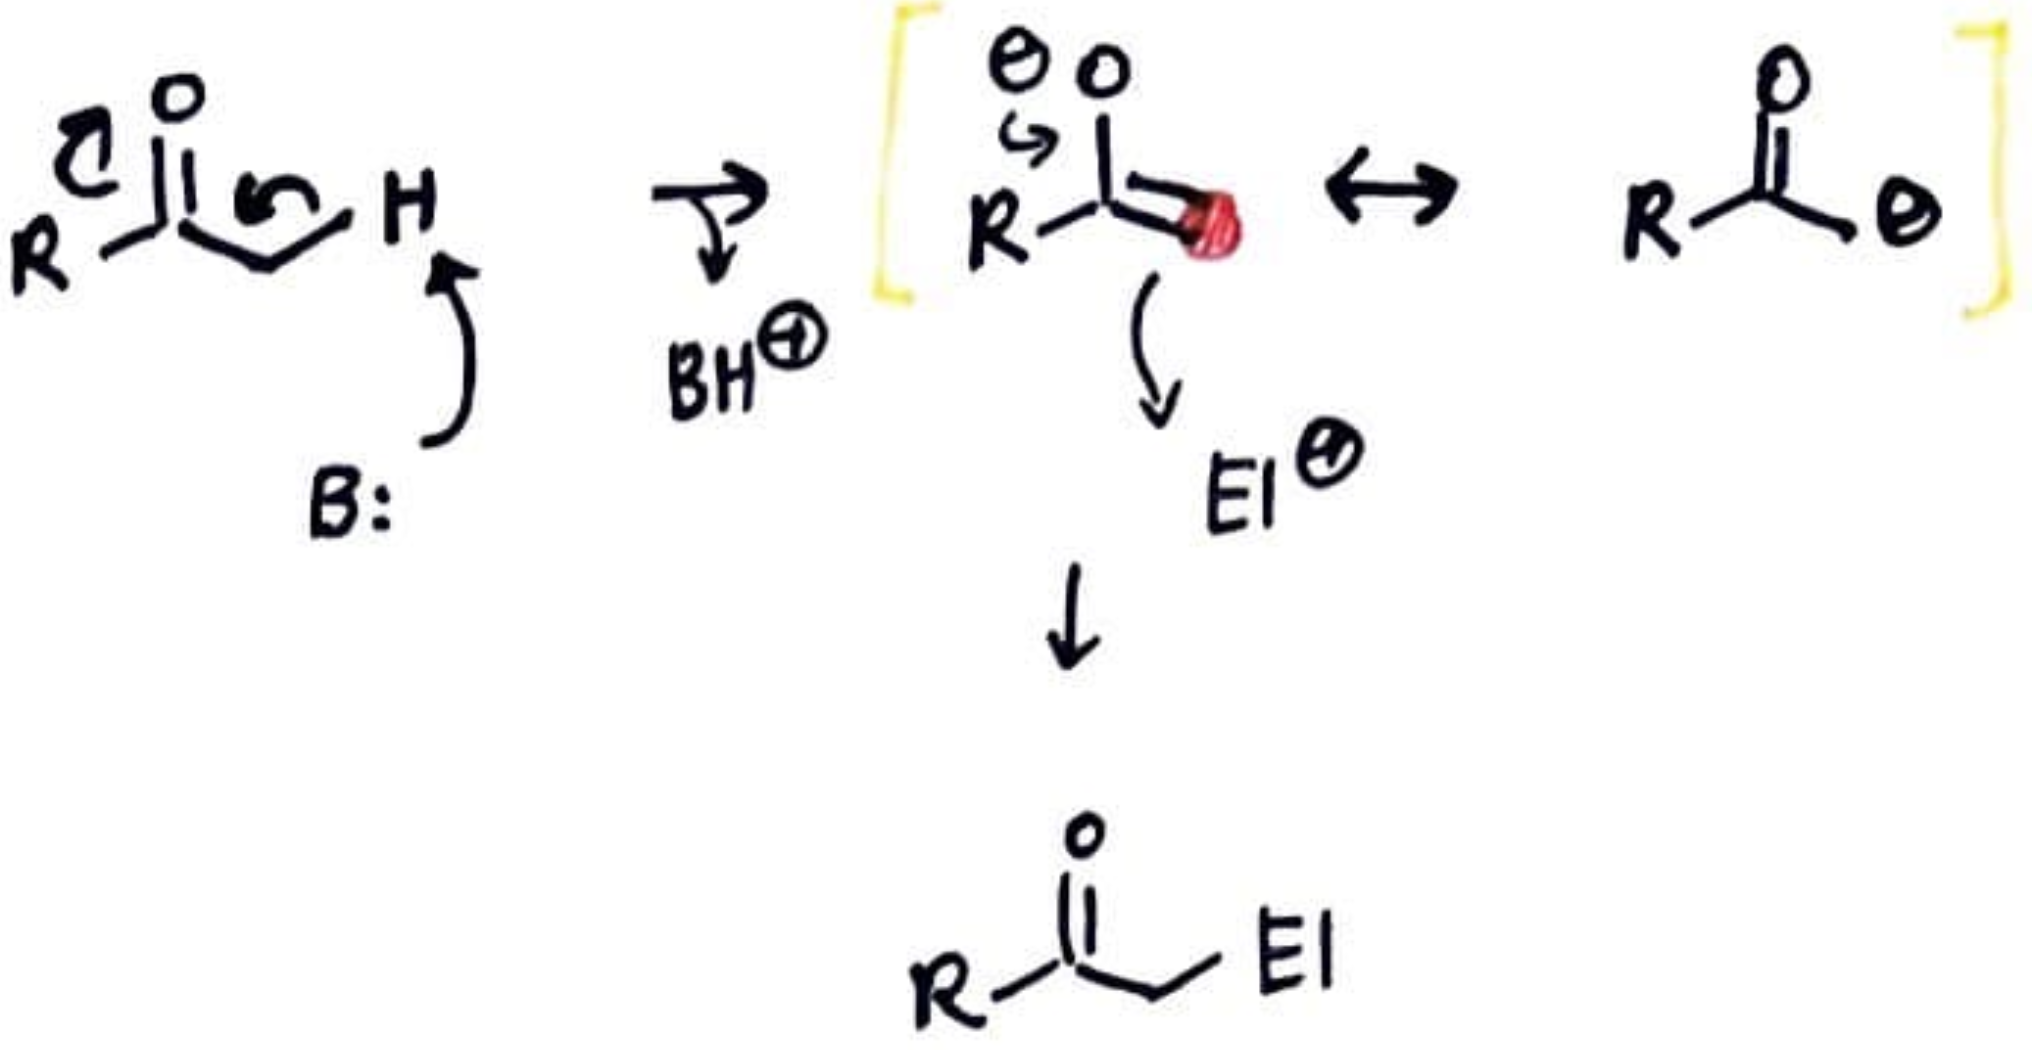
\includegraphics[width=0.9\linewidth]{carbonylRxnb.png}
            \caption{As nucleophile.}
            \label{fig:carbonylRxnb}
        \end{subfigure}
        \caption{Carbonyl-based chemical reactions.}
        \label{fig:carbonylRxn}
    \end{figure}
    \begin{itemize}
        \item Carbonyls have two important modes of reactivity.
        \item We've already discussed how carbonyls can act as electrophiles (Figure \ref{fig:carbonylRxna}).
        \begin{itemize}
            \item This yields a tetrahedral intermediate, as we've discussed.
        \end{itemize}
        \item The other mode of reactivity --- which is new and our focus --- is that we can deprotonate at the $\alpha$-carbon to make a nucleophilic species (Figure \ref{fig:carbonylRxnb}).
        \begin{itemize}
            \item The major resonance structure will be the oxygen-centered one (because oxygen is more electronegative).
            \item However, most reactions we're interested in proceed at carbon.
        \end{itemize}
    \end{itemize}
    \item Key concept: Oxygen \emph{enables} this mode of reactivity stabilizing the negative charge.
    \begin{figure}[h!]
        \centering
        \begin{subfigure}[b]{0.25\linewidth}
            \centering
            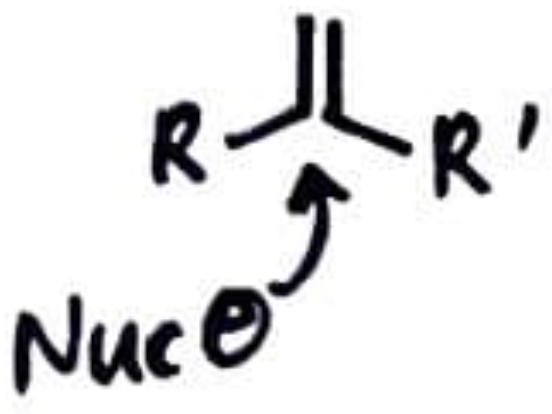
\includegraphics[width=0.38\linewidth]{alkeneCarbonyla.png}
            \caption{Not as electrophiles.}
            \label{fig:alkeneCarbonyla}
        \end{subfigure}
        \begin{subfigure}[b]{0.25\linewidth}
            \centering
            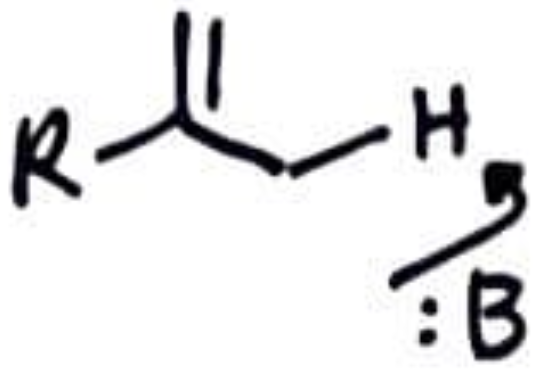
\includegraphics[width=0.38\linewidth]{alkeneCarbonylb.png}
            \caption{Not as nucleophiles.}
            \label{fig:alkeneCarbonylb}
        \end{subfigure}
        \caption{Alkenes do not react via carbonyl-analogous pathways.}
        \label{fig:alkeneCarbonyl}
    \end{figure}
    \begin{itemize}
        \item For the purposes of 5.13, analogous addition to alkenes (Figure \ref{fig:alkeneCarbonyla}) and $\alpha$-deprotonation of alkenes (Figure \ref{fig:alkeneCarbonylb}) is very rare.
    \end{itemize}
    \item Let's now discuss tautomers.
    \begin{figure}[h!]
        \centering
        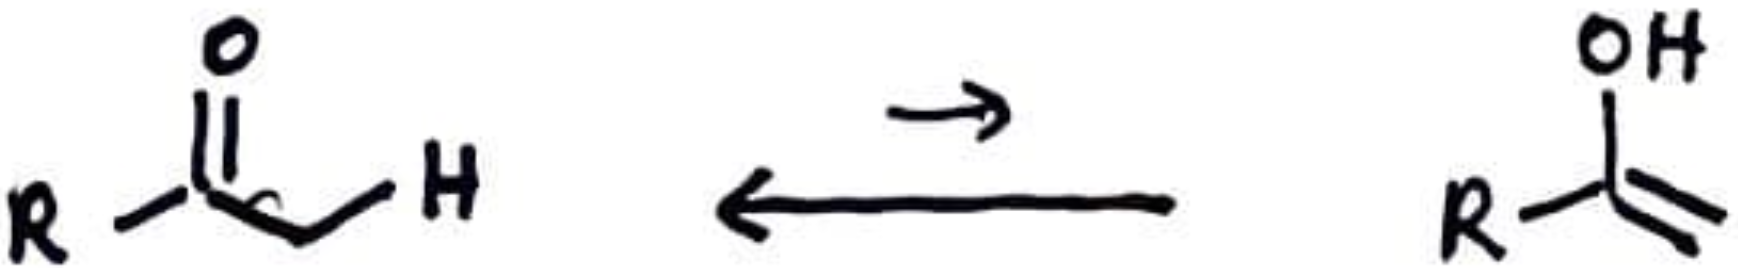
\includegraphics[width=0.32\linewidth]{ketoEnol.png}
        \caption{Keto-enol tautomerization.}
        \label{fig:ketoEnol}
    \end{figure}
    \begin{itemize}
        \item Ketones can tautomerize to \textbf{enols} (a portmanteau of alk\underline{en}e and alcoh\underline{ol}).
        \item The keto and enol form are known as \textbf{tautomers}.
        \item The equilibrium favors the keto form by far (about a million to one; we'll only have $0.001\%$ enol).
    \end{itemize}
    \item Catalysts can speed up the inverconversion, but they can't change the equilibrium.
    \begin{itemize}
        \item Let's discuss the mechanism by which bases and acids speed this process up, though.
    \end{itemize}
    \pagebreak
    \item Base-catalyzed keto-enol tautomerization mechanism.
    \begin{figure}[h!]
        \centering
        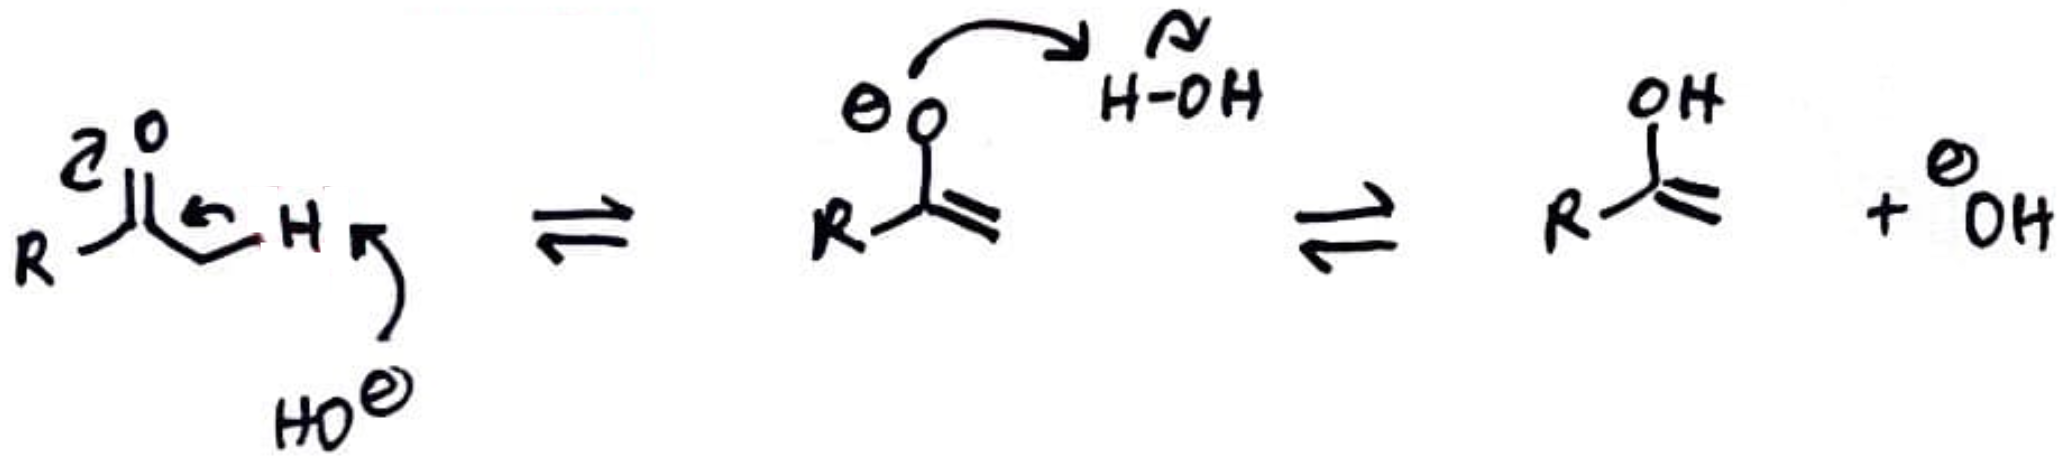
\includegraphics[width=0.55\linewidth]{ketoEnolBase.png}
        \caption{Keto-enol tautomerization mechanism (base-catalyzed).}
        \label{fig:ketoEnolBase}
    \end{figure}
    \begin{itemize}
        \item The $\alpha$-carbon of a ketone has $\pKa\approx 20$.
        \begin{itemize}
            \item This is a good number to memorize, not because you'll ever be tested on it but because understanding relative $\pKa$'s will aid your chemical intuition.
        \end{itemize}
        \item Hydroxide can speed up this process by deprotonating the $\alpha$-carbon.
        \begin{itemize}
            \item Then we just protonate the oxygen.
        \end{itemize}
        \item Recall that we still have $\Keq\ll 1$.
    \end{itemize}
    \item Acid-catalyzed keto-enol tautomerization mechanism.
    \begin{figure}[h!]
        \centering
        \begin{subfigure}[b]{\linewidth}
            \centering
            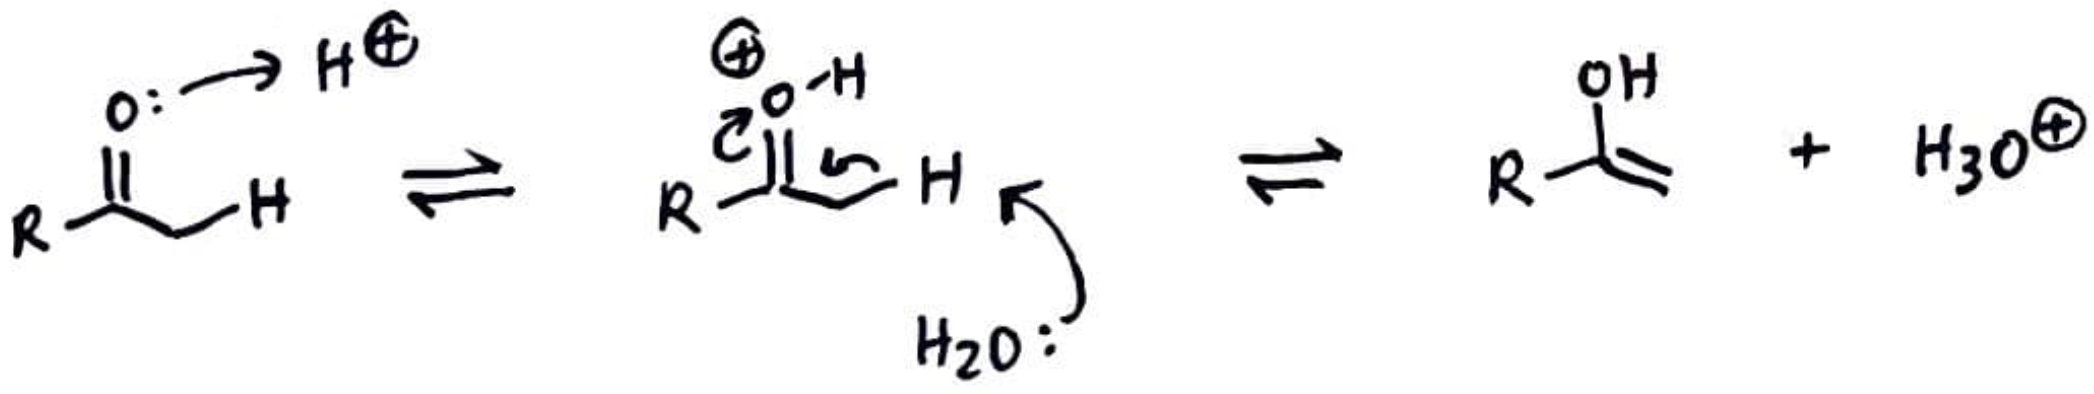
\includegraphics[width=0.62\linewidth]{ketoEnolAcida.png}
            \caption{Correct mechanism.}
            \label{fig:ketoEnolAcida}
        \end{subfigure}\\[2em]
        \begin{subfigure}[b]{\linewidth}
            \centering
            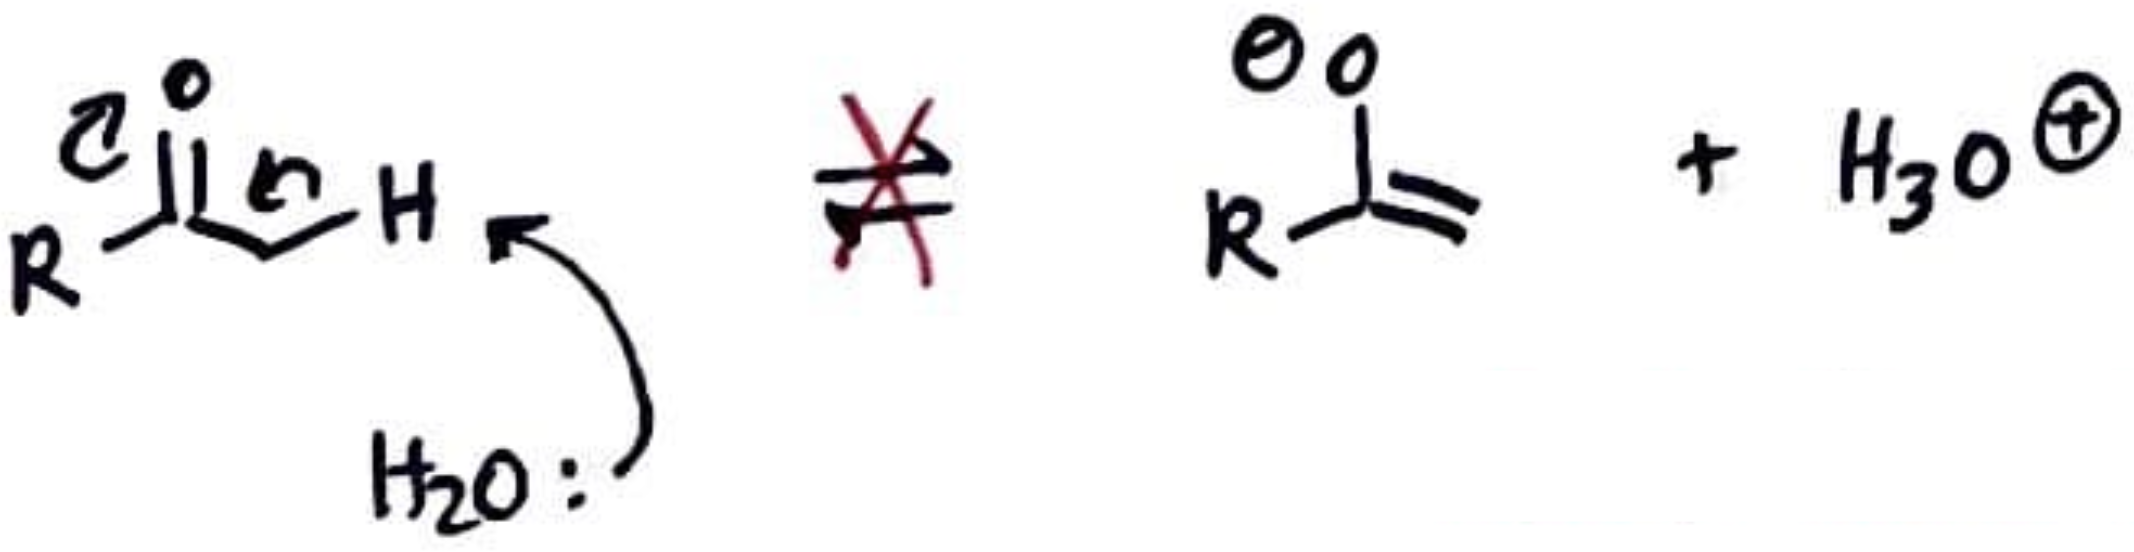
\includegraphics[width=0.4\linewidth]{ketoEnolAcidb.png}
            \caption{Incorrect mechanism.}
            \label{fig:ketoEnolAcidb}
        \end{subfigure}
        \caption{Keto-enol tautomerization mechanism (acid-catalyzed).}
        \label{fig:ketoEnolAcid}
    \end{figure}
    \begin{itemize}
        \item We can either write the reagents equivalently as \ce{H+}/\ce{H2O} or \ce{H3O+}.
        \item As we've been doing, we begin by protonating the carbonyl.
        \item Then the best base in solution comes and deprotonates the $\alpha$-carbon.
        \begin{itemize}
            \item Water isn't a great base, but it's all we've got.
        \end{itemize}
        \item Note that we do \emph{not} do deprotonation first and protonation second, as drawn in Figure ??b.
        \begin{itemize}
            \item Remember that anions cannot exist in acidic solution!
        \end{itemize}
    \end{itemize}
    \item So this is all great, but what if we don't believe Prof. Buchwald that tautomerization occurs?
    \begin{itemize}
        \item It's good to question things in science!
        \item Many times, we've assumed things that later experiments have proven incorrect.
    \end{itemize}
    \pagebreak
    \item We can find evidence for enolization via an isotopic labeling study.
    \begin{figure}[h!]
        \centering
        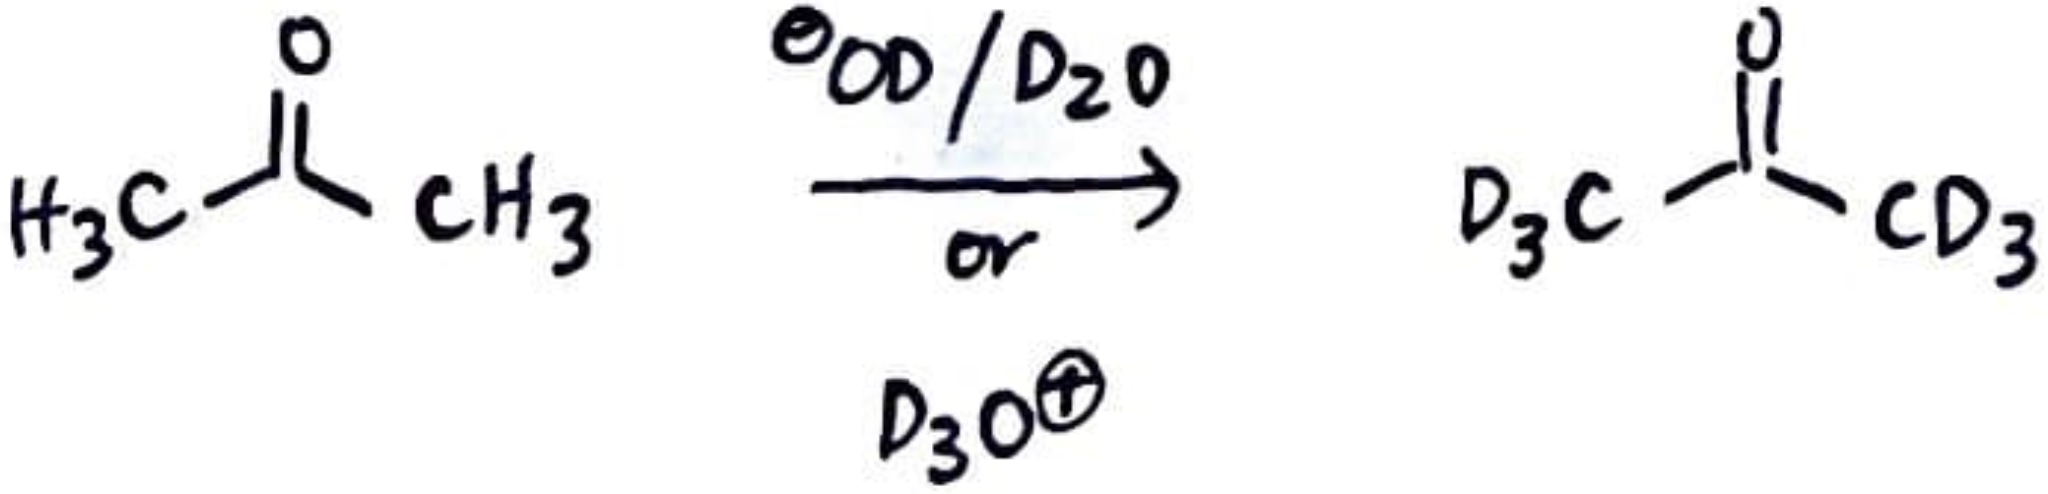
\includegraphics[width=0.4\linewidth]{ketoEnolIsotope.png}
        \caption{Isotopic labeling provides evidence for keto-enol tautomerization.}
        \label{fig:ketoEnolIsotope}
    \end{figure}
    \begin{itemize}
        \item If we dissolve acetone in basic deuterated water and deuteroxide (or acid), we will eventually obtain deuteroacetone.
        \item The mechanism proceeds analogously to Figure \ref{fig:ketoEnolBase} or \ref{fig:ketoEnolAcida}, except that our reagents are all \ce{DO-} and \ce{D2O}.
        \begin{itemize}
            \item In particular, we replace each of the six hydrogens one at a time with deuterium, eventually leading to the product.
            \item We form the fully deuterated product instead of a \ce{H}/\ce{D}-mixed product because we assume that the concentration of deuterated acid or base and water is \emph{much} greater than the concentration of acetone. This is similar to the swamping effect in Figure \ref{fig:transesterEqa}.
        \end{itemize}
    \end{itemize}
    \item We now move onto Topic B: $\alpha$-halogenation of ketones.
    \begin{itemize}
        \item We can do this with chlorine, bromine, or iodine.
    \end{itemize}
    \item Base-promoted $\alpha$-halogenation mechanism.
    \begin{figure}[h!]
        \centering
        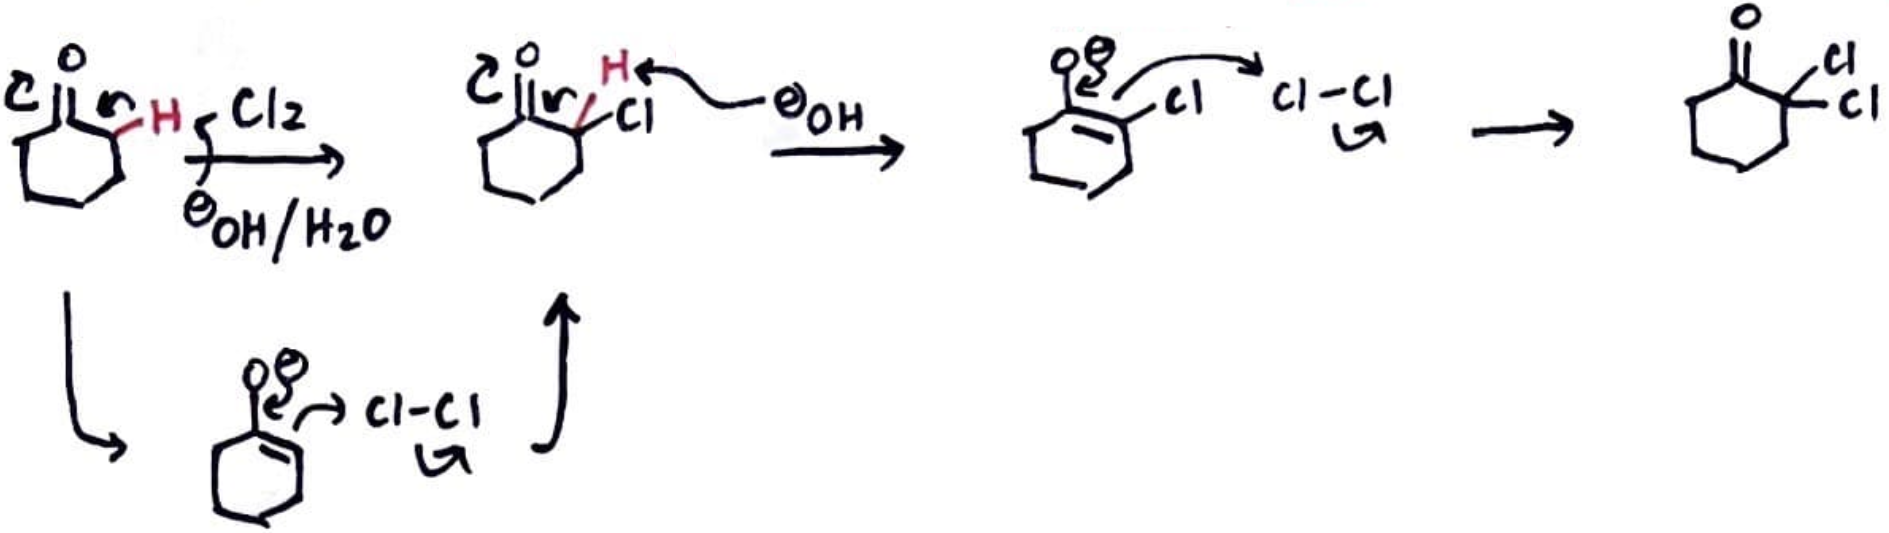
\includegraphics[width=0.8\linewidth]{alphaHaloBase.png}
        \caption{$\alpha$-halogenation mechanism (base-promoted).}
        \label{fig:alphaHaloBase}
    \end{figure}
    \begin{itemize}
        \item Imagine we mix cyclohexanone with chlorine gas under basic conditions. What's going to happen?
        \item We'll form a small amount of enolate, and then chlorinate to form $\alpha$-chlorocyclohexanone.
        \begin{itemize}
            \item We declare victory!
            \item Except that the world is a harsh place and --- like in Figure \ref{fig:redAmin12a} --- we can get further reactivity.
        \end{itemize}
        \item In particular, the hydrogen geminal to the $\alpha$-chlorine is now \emph{more} acidic (proximity to an EWG, so anion is stabilized).
        \begin{itemize}
            \item Thus, we can react again to get $\alpha$-dichlorocyclohexanone.
        \end{itemize}
        \item Thus, this reaction is not good\dots except in one case.
    \end{itemize}
    \pagebreak
    \item The iodoform reaction.
    \begin{figure}[h!]
        \centering
        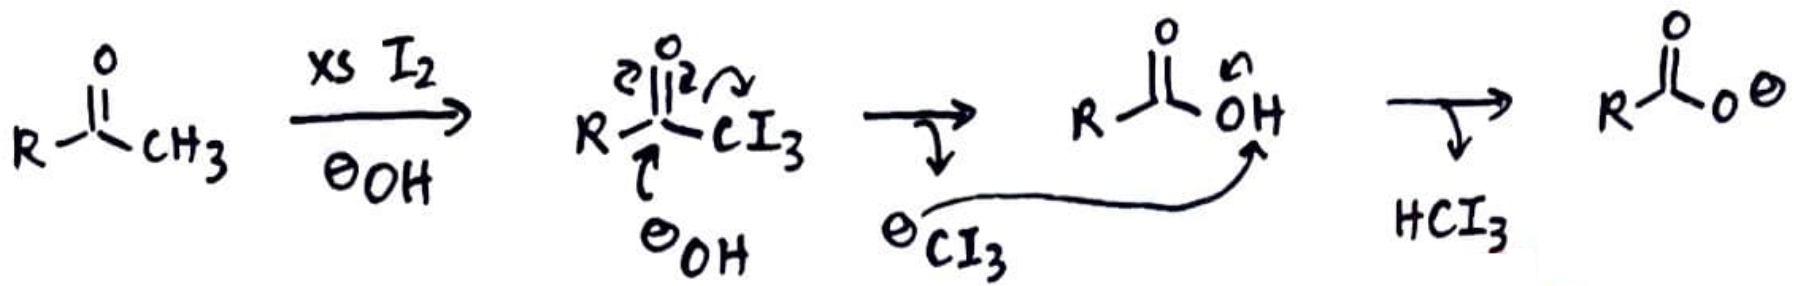
\includegraphics[width=0.7\linewidth]{iodoform.png}
        \caption{Iodoform reaction.}
        \label{fig:iodoform}
    \end{figure}
    \begin{itemize}
        \item In the first step, we have three successive iodinations to yield the triiodomethylketone.
        \item This is such a strong EWG and good leaving group that the triiodomethylketone acts kind of like an acid chloride.
        \begin{itemize}
            \item In particular, we get an addition-elimination mechanism that kicks out the triiodomethanide anion.
            \item This anion can then be protonated by the resultant carboxylic acid to yield iodoform (\ce{HCI3}) and a stable carboxylate.
        \end{itemize}
        \item Iodoform precipitates as a yellow solid.
        \begin{itemize}
            \item In the olden days, it used to be a test for a ketone.
            \item Before we had NMR, mass spec, and other kinds of spectroscopy, we had a bunch of test reagents that we would add to our compounds to determine what it was.
            \item Essentially, if we had a compound and we didn't know what it was but thought it was a ketone, we could confirm or deny this by adding iodine and base to our mixture!
        \end{itemize}
    \end{itemize}
    \item What does it mean when Prof. Buchwald draws a circular arrow from a carbonyl $\pi$-bond back to it?
    \begin{itemize}
        \item They use this in \textcite{bib:Clayden}!
        \item This is a shorthand for the two-step addition-elimination process, in which electrons kick up in a first step and then kick back down in a second step.
        \item This is similar to how we shorthand a two-step proton transfer as "PT!"
    \end{itemize}
    \item So how do we make mono-$\alpha$-haloketones, if that's our goal?
    \begin{itemize}
        \item Use acid-catalyzed $\alpha$-halogenation!
    \end{itemize}
    \item Acid-catalyzed $\alpha$-halogenation mechanism.
    \begin{figure}[h!]
        \centering
        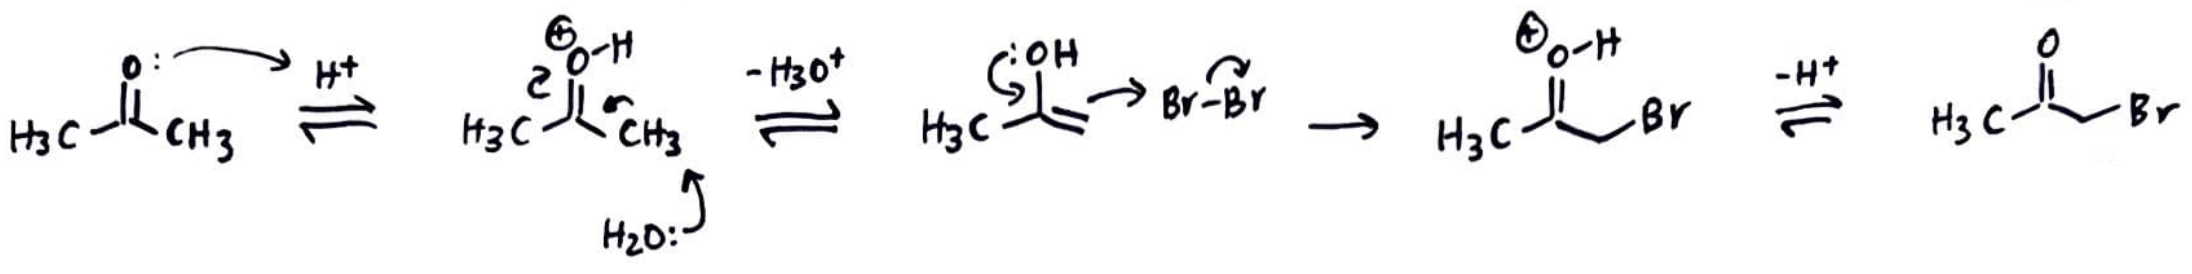
\includegraphics[width=\linewidth]{alphaHaloAcid.png}
        \caption{$\alpha$-halogenation mechanism (acid-catalyzed).}
        \label{fig:alphaHaloAcid}
    \end{figure}
    \begin{itemize}
        \item Acids encourage the rate of formation of the enol.
        \item Then if we do this in the presence of bromine, we'll get $\alpha$-bromoacetone (following deprotonation).
        \item Now the product is \emph{less} reactive than the starting material (because the bromine EWG stabilizes the carbonyl and disfavors protonation of it).
        \item Takeaway: Acid-catalyzed $\alpha$-halogenation is selective for monohalogenation.
        \item This process is used to synthesize a lot of medicines and drug molecules.
    \end{itemize}
    \pagebreak
    \item We now move onto Topic C: $\alpha$-alkylation.
    \begin{itemize}
        \item This is the heavy hitter; a really, really important reaction of ketones.
    \end{itemize}
    \item General form.
    \begin{figure}[h!]
        \centering
        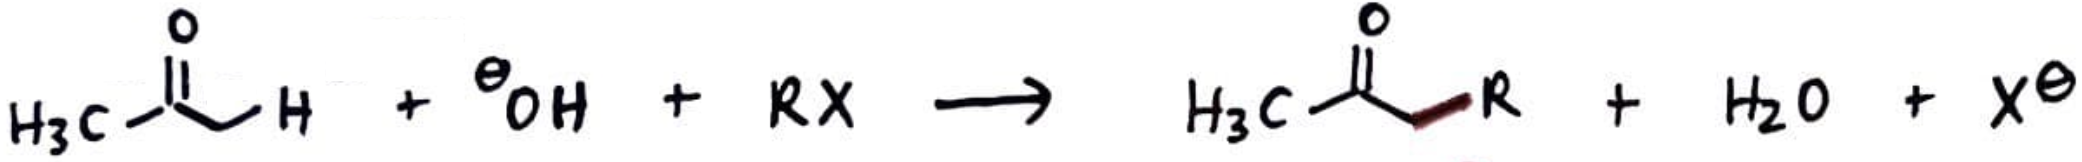
\includegraphics[width=0.65\linewidth]{alphaAlk.png}
        \caption{$\alpha$-alkylation.}
        \label{fig:alphaAlk}
    \end{figure}
    \begin{itemize}
        \item Suppose we want to convert a ketone into a new compound where we've formed a \ce{C-C} bond.
        \item The other reagent is a primary or secondary alkyl halide.
    \end{itemize}
    \item Drawing a mechanism for this doesn't seem too bad at first.
    \begin{itemize}
        \item We may deprotonate to the enolate and attack the alkyl halide to start.
        \item But there is a complication.
        \begin{itemize}
            \item We get lots of side reactions!
        \end{itemize}
        \item In 5.13, we're all about efficiency and elegance, so this is not good.
    \end{itemize}
    \item There are several solutions to this issue, which we'll discuss presently.
    \item Solution 1: Use lithium diisopropylamide (LDA).
    \begin{figure}[h!]
        \centering
        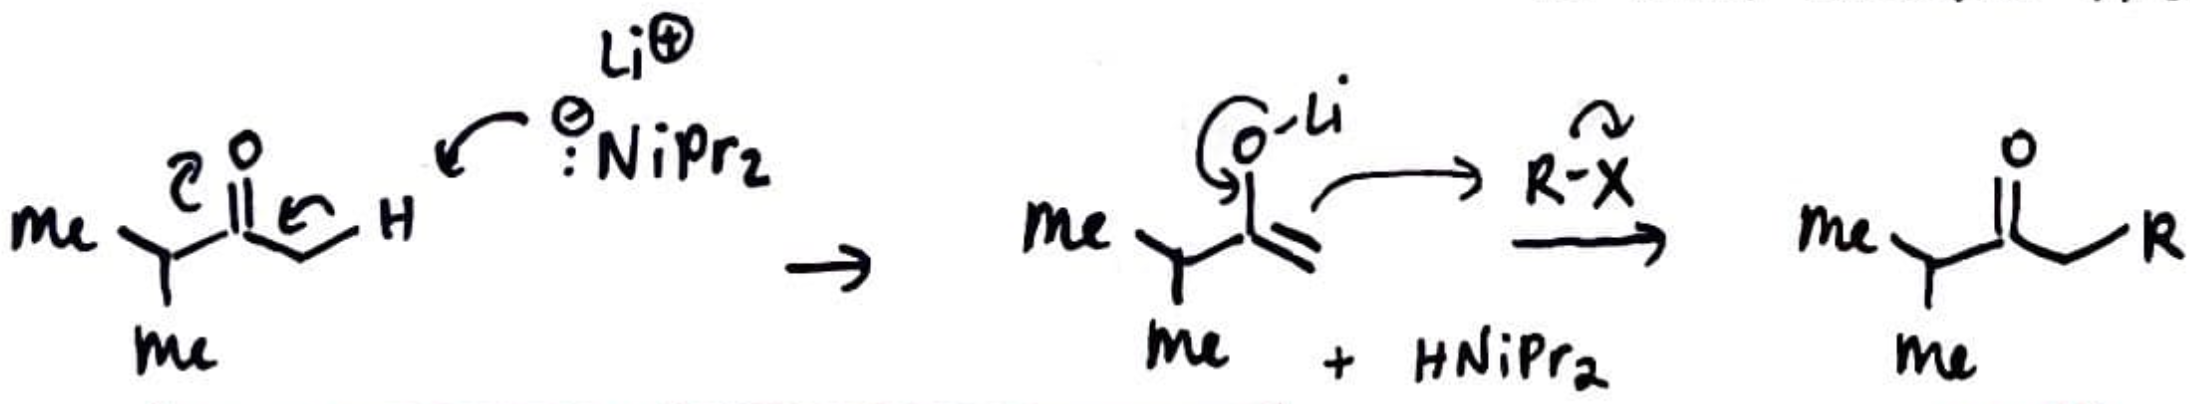
\includegraphics[width=0.6\linewidth]{alphaAlkLDA.png}
        \caption{$\alpha$-alkylation with lithium diisopropylamide.}
        \label{fig:alphaAlkLDA}
    \end{figure}
    \begin{itemize}
        \item See Figure \ref{fig:amineEx2b} for the structure and synthesis of LDA.
        \item Helpful characteristics of LDA.
        \begin{itemize}
            \item LDA is a strong base.
            \item It is secondary and hence hindered (therefore a poor nucleophile).
            \item The conjugate acid of LDA has $\pKa\approx 35$.
            \item Thus, it will only deprotonate and not do any competitive addition chemistry!
        \end{itemize}
        \item We begin with an essentially irreversible deprotonation to the enolate.
        \item This is followed by 100\% conversion to the alkylated product.
    \end{itemize}
    \item Using LDA is a relatively modern solution --- only about 50 years old.
    \begin{itemize}
        \item However, organic chemistry has been around for close to 250 years!
        \item The roots of organic chemistry are in the old German dye industry, which morphed into the present-day pharmaceutical industry.
        \item So how did people do this stuff before LDA? Via solution 2.
    \end{itemize}
    \pagebreak
    \item Solution 2: Malonate ester synthesis.
    \begin{figure}[h!]
        \centering
        \begin{subfigure}[b]{\linewidth}
            \centering
            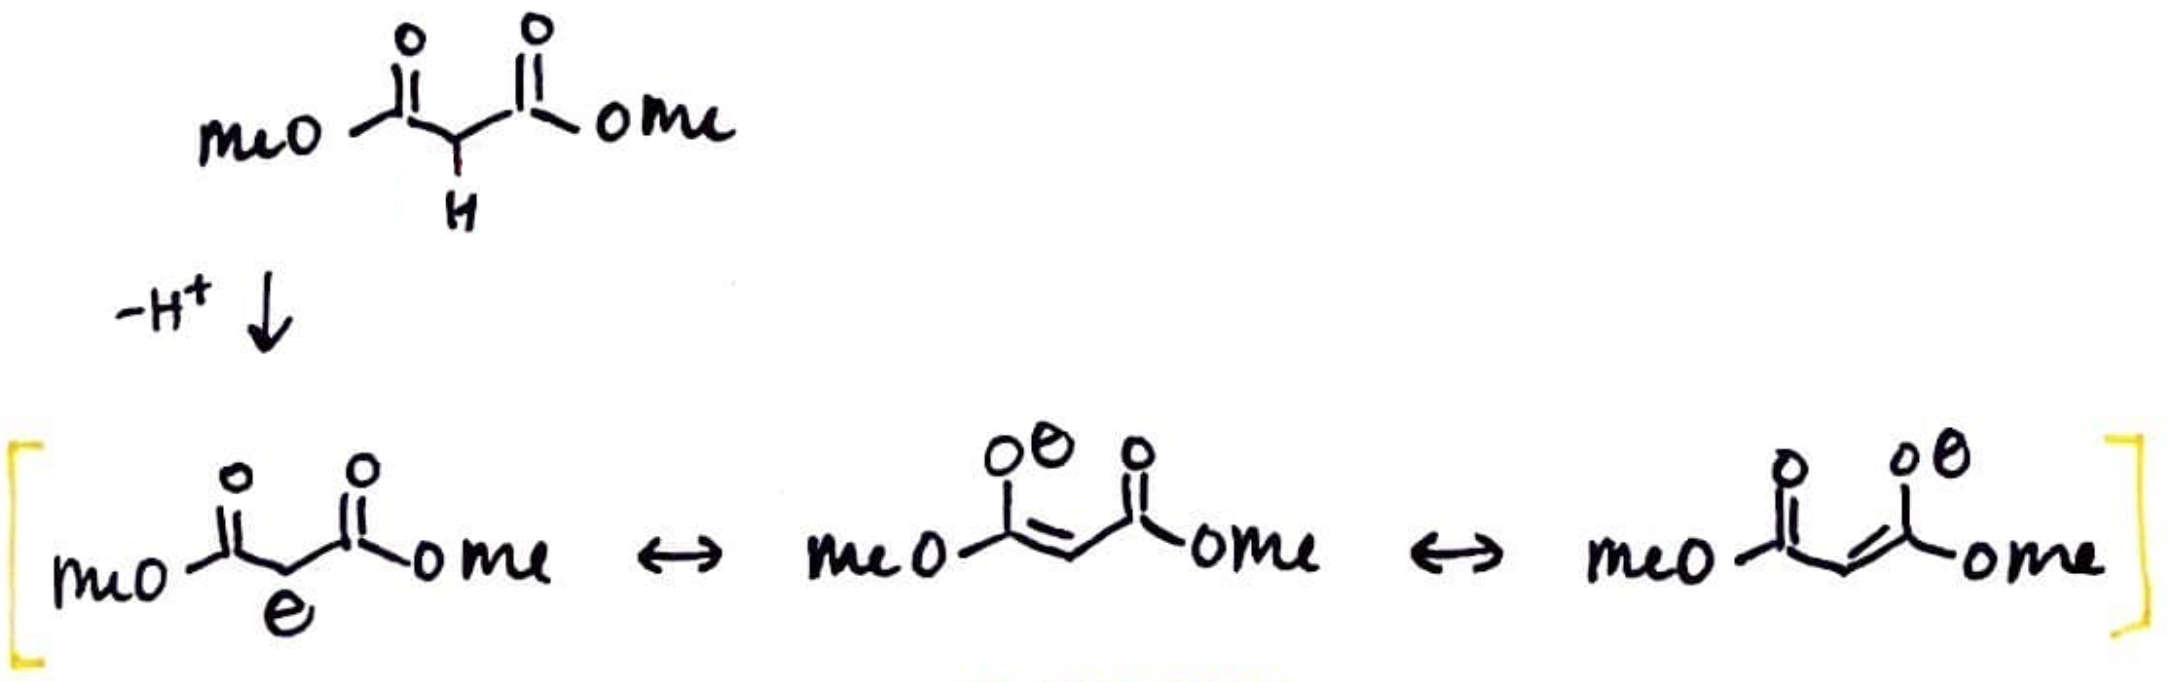
\includegraphics[width=0.6\linewidth]{alphaAlkMalEstera.png}
            \caption{Malonate ester resonance.}
            \label{fig:alphaAlkMalEstera}
        \end{subfigure}\\[2em]
        \begin{subfigure}[b]{\linewidth}
            \centering
            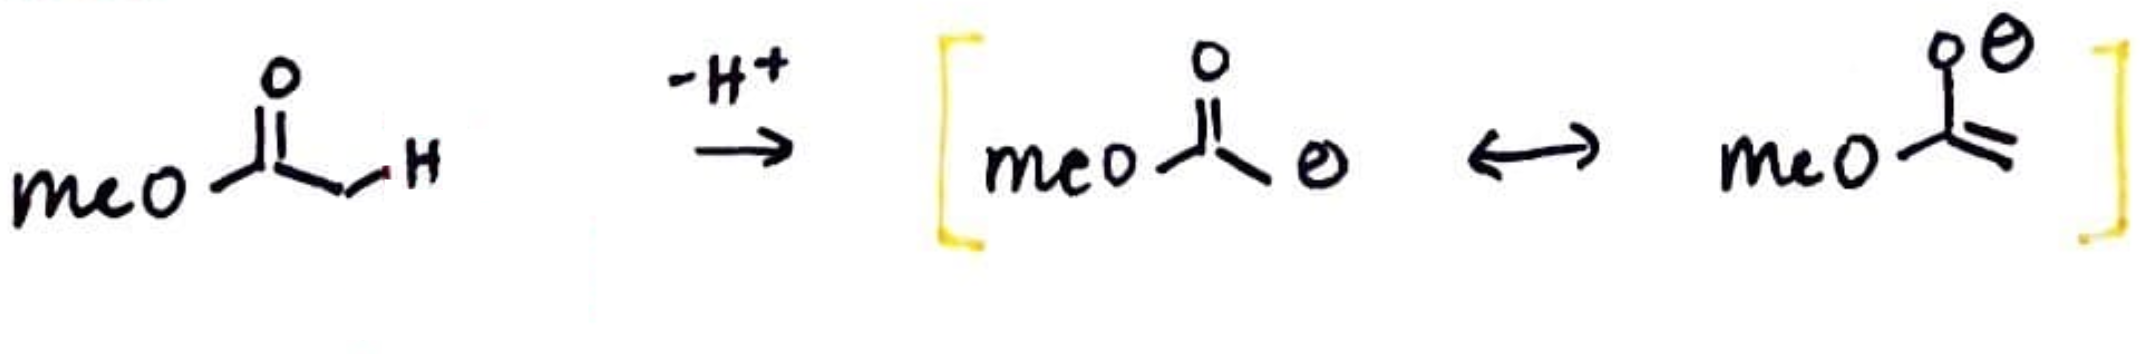
\includegraphics[width=0.5\linewidth]{alphaAlkMalEsterb.png}
            \caption{Regular ester resonance.}
            \label{fig:alphaAlkMalEsterb}
        \end{subfigure}
        \caption{$\alpha$-alkylation with malonate esters.}
        \label{fig:alphaAlkMalEster}
    \end{figure}
    \begin{itemize}
        \item The starting material has esters on both sides (either ethyl or methyl; it doesn't matter).
        \item The important thing is that for the malonate ester, $\pKa\approx 13$.
        \begin{itemize}
            \item In contrast, a regular ester has $\pKa\approx 25$.
        \end{itemize}
        \item Why this drastic difference in $\pKa$?
        \begin{itemize}
            \item The deprotonated malonate ester's anion has more resonance forms (two adjacent carbonyls into which to delocalze!) than the deprotonated ester (only one adjacent carbonyl).
        \end{itemize}
        \item This difference leads us to call the deprotonated malonate ester a \textbf{soft enolate}.
        \begin{itemize}
            \item These characteristics make it very easy and safe to work with, so it's often used at scale.
        \end{itemize}
    \end{itemize}
    \item We'll now quickly introduce a topic that we'll also discuss more next time.
    \item Kinetic vs. thermodynamic enolates.
    \item \textbf{Kinetic} (enolate): The enolate generated by deprotonation at the less-substituted position, all else being equal.
    \item Example: LDA (really big and bulky) will selectively form the kinetic enolate at the unsubstituted position of $\alpha$-methylcyclohexanone.
    \begin{figure}[h!]
        \centering
        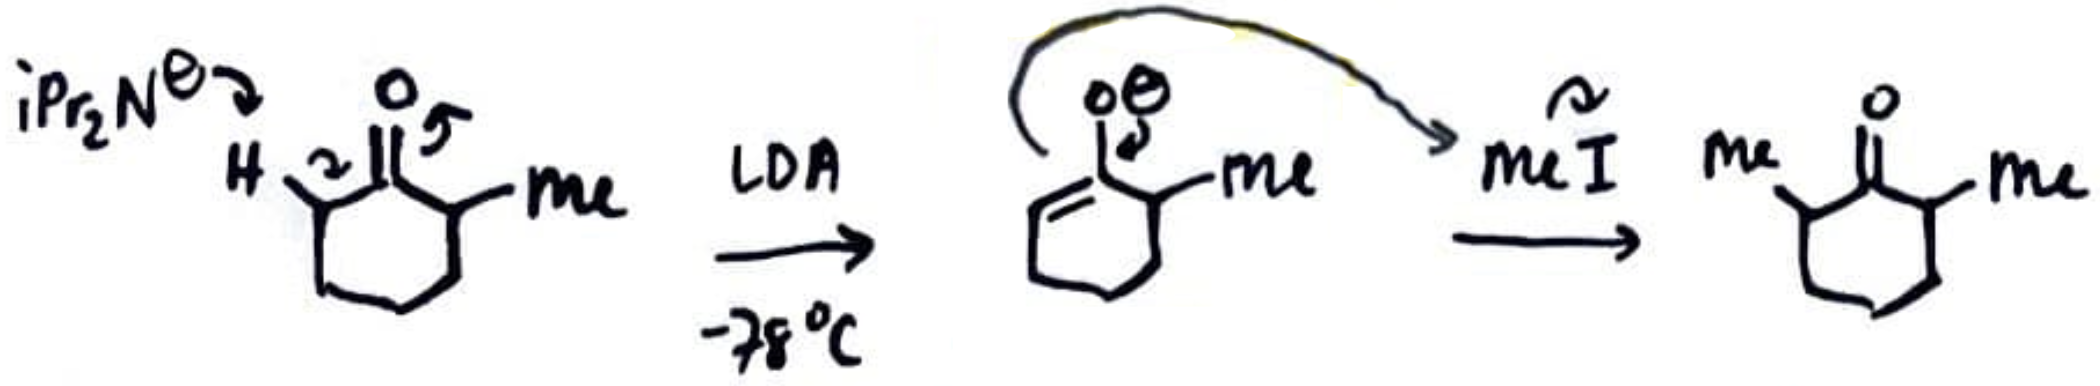
\includegraphics[width=0.6\linewidth]{enolateKinetic.png}
        \caption{Kinetic enolate formation.}
        \label{fig:enolateKinetic}
    \end{figure}
    \begin{itemize}
        \item This enolate could then be used --- for example --- to attack methyl iodide (\ce{MeI}) and alkylate.
        \item Note that this process would most likely form a mixture of stereoisomers.
    \end{itemize}
    \pagebreak
    \item \textbf{Thermodynamic} (enolate): The enolate that is more stable.
    \item Example: Potassium \emph{t}-butoxide (\ce{KO{}^{\emph{t}}Bu}) has $\pKa\approx\text{\numrange{16}{18}}$, so it deprotonates $\alpha$-methylcyclohexanone reversibly until we get the more stable one.
    \begin{figure}[h!]
        \centering
        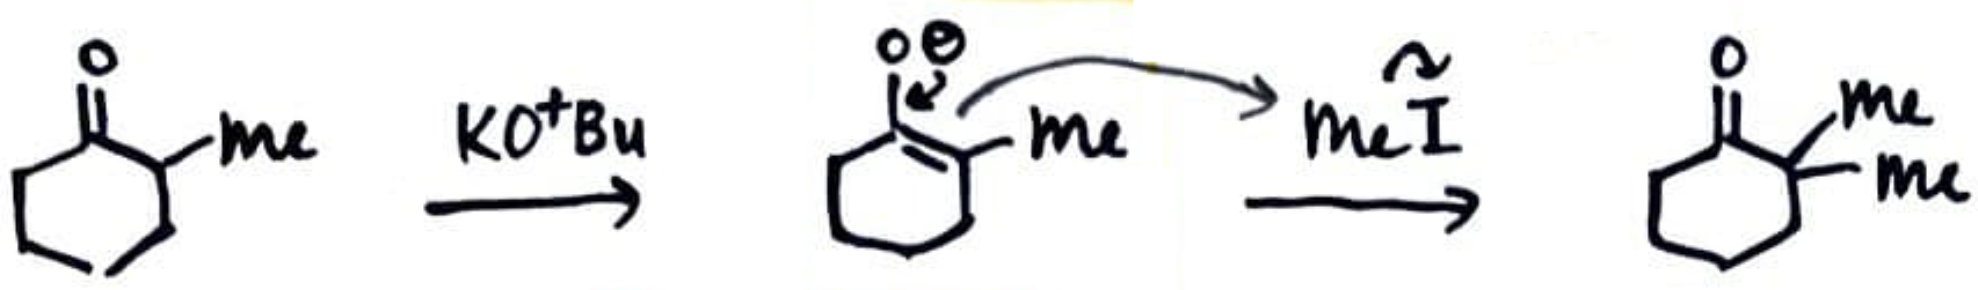
\includegraphics[width=0.55\linewidth]{enolateThermodynamic.png}
        \caption{Thermodynamic enolate formation.}
        \label{fig:enolateThermodynamic}
    \end{figure}
    \begin{itemize}
        \item Treating this with \ce{MeI} then generates the $\alpha$-dimethylated form of cyclohexanone.
    \end{itemize}
    \item You can add in \ce{Me3SiCl} to trap enolates the silyl enol ether.
    \begin{figure}[h!]
        \centering
        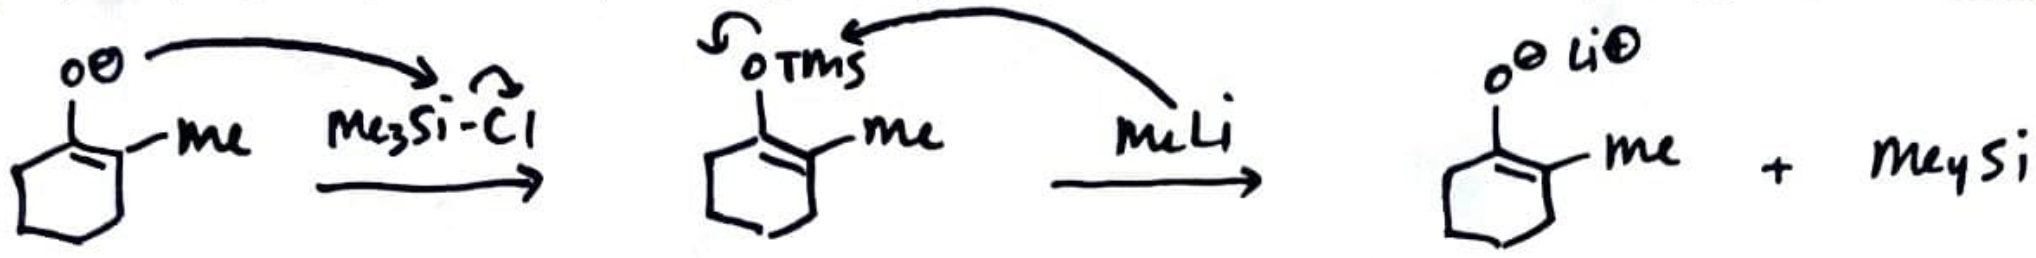
\includegraphics[width=0.75\linewidth]{enolateTMS.png}
        \caption{Trapping enolates as silyl enol ethers.}
        \label{fig:enolateTMS}
    \end{figure}
    \begin{itemize}
        \item This silyl protecting group could then be removed with \ce{MeLi}, regenerating the enolate and yielding tetramethylsilane (\ce{SiMe4}) as a byproduct.
        \item In the deprotection step, the methyl anion attacks the silicon atom in the TMS group, engaging in an S\textsubscript{N}2 displacement.
    \end{itemize}
\end{itemize}



\section{Enolate Alkylation}
\begin{itemize}
    \item \marginnote{11/18:}We will not begin with a line-by-line review of last lecture; rather, we will clarify some things.
    \item Lecture 29 recap.
    \begin{itemize}
        \item Recall kinetic vs. thermodynamic enolates (Figures \ref{fig:enolateKinetic} \& \ref{fig:enolateThermodynamic}).
        \item When we use a strong, hindered base (like \ce{LDA}), we abstract the unhindered proton to form the kinetic enolate.
        \begin{itemize}
            \item This process is irreversible, and yields 100\% of the kinetic enolate.
            \item The process is irreversible because $\pKa\approx 35$ for the conjugate acid of LDA (lithium diisopropylamine), so this conjugate acid cannot react backwards.
        \end{itemize}
        \item Use of a somewhat strong, somewhat bulky base (like \ce{KO{}^{\emph{t}}Bu} in \ce{{}^{\emph{t}}BuOH}).
        \begin{itemize}
            \item This process is highly reversible, so we'll abstract the unhindered proton first. But then the enolate can react backwards with \ce{{}^{\emph{t}}BuOH} to reform the ketone!
            \item This process is highly reversible because $\pKa\approx 19$ for \ce{{}^{\emph{t}}BuOH}, so this conjugate acid \emph{can} react backwards.
            \item However, when we eventually deprotonate the hindered proton, we form a more stable enolate that is \emph{less likely} to react backwards.
            \item Thus, the net result is that we form the \emph{thermodynamic} enolate under these conditions.
        \end{itemize}
        \item Both of these enolates can then be trapped with \ce{MeI} into the corresponding $\alpha$-alkylation product.
    \end{itemize}
    \pagebreak
    \item Lecture outline.
    \begin{enumerate}[label={\Alph*.},start=3]
        \item $\alpha$-alkylation.
        \begin{itemize}
            \item Enolate-forming bases.
            \item Enolates from esters (hard to form) and aldehydes (don't form).
            \item Enolate-alkylation electrophiles.
            \item Synthesis of $\alpha$-substituted acetic acid derivatives.
            \item Synthesis of $\alpha$-substituted 1,3-diols.
        \end{itemize}
    \end{enumerate}
    \item We return to Topic C: $\alpha$-alkylation.
    \item Let's consider the properties of several strong bases.
    \begin{table}[h!]
        \centering
        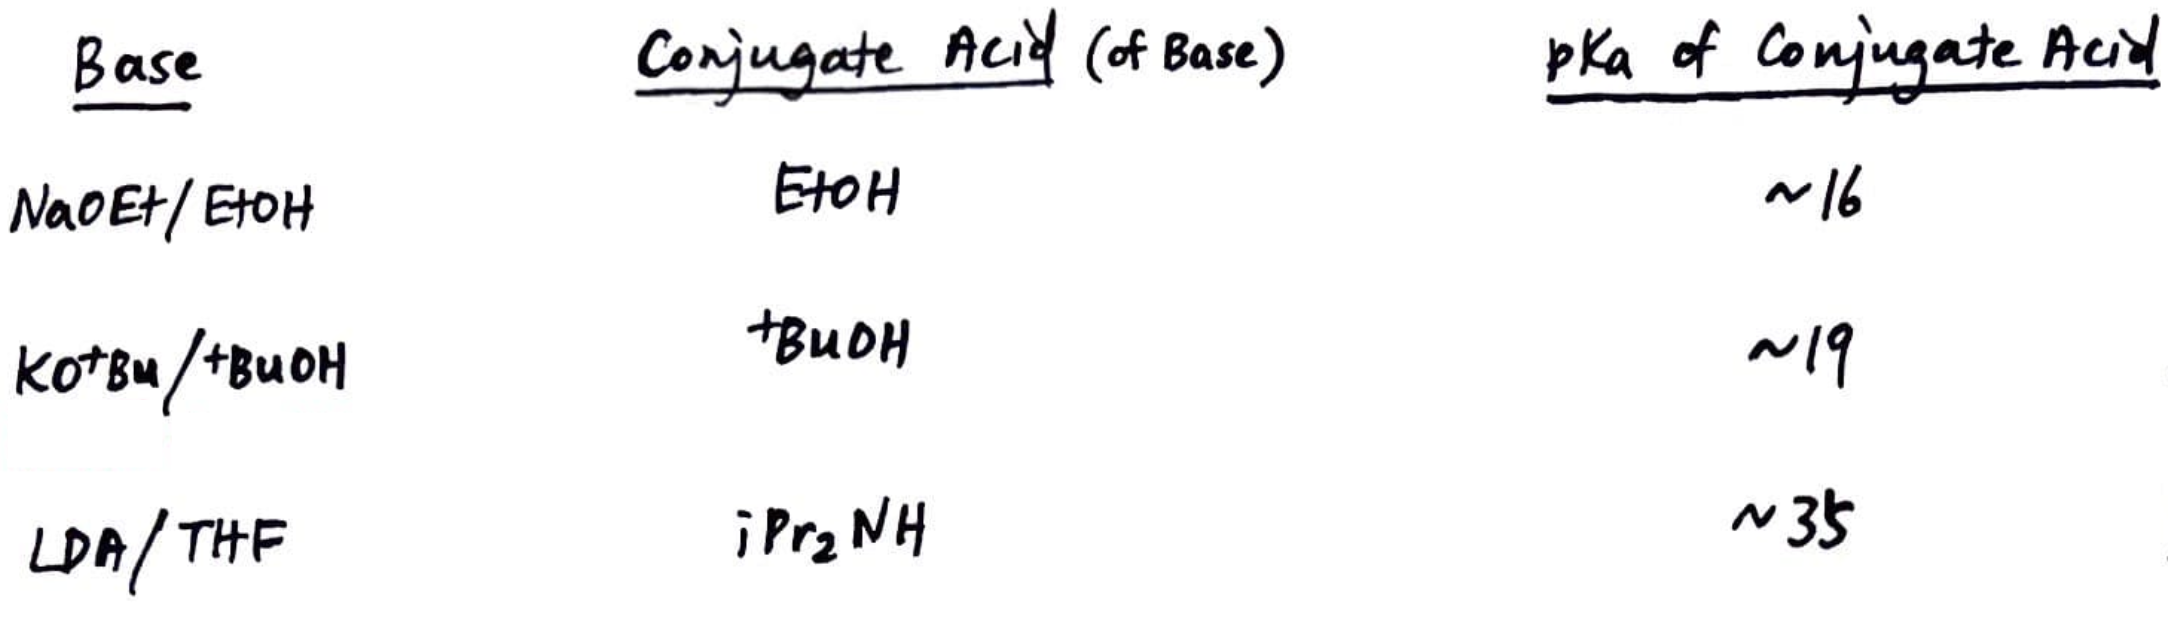
\includegraphics[width=0.6\linewidth]{enolateBase.png}
        \caption{$\pKa$'s of typical enolate-forming bases.}
        \label{tab:enolateBase}
    \end{table}
    \begin{itemize}
        \item The left column shows a base and the solvent in which you use it, not necessarily the base and it's conjugate acid!
        \item It follows from the table that \ce{NaOEt} and \ce{KO{}^{\emph{t}}Bu} are reversible bases, and LDA is an irreversible base.
        \item The difference between the first two is that \ce{KO{}^{\emph{t}}Bu} is bulkier and less nucleophilic.
        \begin{itemize}
            \item So if we're worried about nucleophilic attack as a side reaction, use this!
        \end{itemize}
        \item Otherwise, \ce{NaOEt} is cheaper and more pleasant to work with.
    \end{itemize}
    \item So what happens when we do enolate formation with different bases?
    \begin{itemize}
        \item Suppose that the conjugate acid \ce{B1H} has $\pKa>22$.
        \begin{itemize}
            \item Then the reaction is irreversible.
            \item Example: LDA!
        \end{itemize}
        \item Suppose that the conjugate acid \ce{B2H} has $16<\pKa<22$.
        \begin{itemize}
            \item This reaction is reversible.
            \item Examples: \ce{NaOEt} and \ce{KO{}^{\emph{t}}Bu}!
        \end{itemize}
        \item Suppose that the conjugate acid \ce{B3H} has $\pKa<16$.
        \begin{itemize}
            \item Nothing happens! The base isn't strong enough.
        \end{itemize}
        \item Note: We'll read in \textcite{bib:Clayden} that we can use bases with $\pKa<16$ \emph{if} we pair it with a Lewis acid.
        \begin{itemize}
            \item Example: \underline{T}ri\underline{m}ethyl\underline{s}ilyl chloride (\ce{TMSCl}) and \ce{NEt3}.
        \end{itemize}
        \item Generalizing this.
        \begin{itemize}
            \item Consider the $\pKa$ of our $\alpha$-proton.
            \item If the base is 3 $\pKa$ units weaker or stronger, we get reversible enolate formation.
            \item If the base is more than 3 $\pKa$ units stronger, we get irreversible enolate formation.
            \item If the base is more than 3 $\pKa$ units weaker, no reaction occurs because the base is too weak.
        \end{itemize}
    \end{itemize}
    \item Example: Consider methyl isopropyl ketone.
    \begin{itemize}
        \item Use LDA to deprotonate at the methyl group and form the kinetic enolate.
        \item Use \ce{KO{}^{\emph{t}}Bu} in \ce{{}^{\emph{t}}BuOH} to form the thermodynamic enolate.
    \end{itemize}
    \item How about forming enolates from esters?
    \begin{itemize}
        \item We need LDA because $\pKa\approx 25$ for the ester's $\alpha$-proton.
        \item Indeed, esters have significantly less acidic $\alpha$-protons than ketones.
        \item We also need low temperatures to prevent self-condensation.
    \end{itemize}
    \item How about forming enolates from aldehydes?
    \begin{itemize}
        \item For the purposes of this class, we'll say that aldehyde enolates don't exist.
        \item In reality, aldehyde enolates \emph{do} exist, but they are \emph{so} reactive that even at low temperatures, there is lots of competitive self-condensation.
    \end{itemize}
    \item We now return to alkylations of enolates in more depth.
    \begin{itemize}
        \item There are parallels to S\textsubscript{N}2 reactivity here.
        \item Enolates are more hindered than, for example, cyanide nucleophiles (\ce{CN-}), azide nucleophiles (\ce{N3-}), etc.
        \begin{itemize}
            \item They are also more basic.
        \end{itemize}
        \item For the purposes of 5.13\dots
        \begin{itemize}
            \item We'll say that primary alkyl, methyl, benzyl, and allyl halides react with enolates to do $\alpha$-alkylation.
            \begin{itemize}
                \item The TFs will discuss in recitation why benzyl and allyl halides are "activated!!"
            \end{itemize}
            \item We'll also say that secondary alkyl halides do not react with enolates.
            \begin{itemize}
                \item This is because it's more hindered, so we get more competitive elimination.
            \end{itemize}
        \end{itemize}
        \item Tertiary, vinyl, phenyl, and neopentyl halides \emph{never} react with enolates.
        \begin{itemize}
            \item Note that neopentyl is bad (even though it's primary) because it's \emph{super} bulky.
        \end{itemize}
    \end{itemize}
    \item We now discuss the synthesis of $\alpha$-substituted malonate esters.
    \begin{figure}[h!]
        \centering
        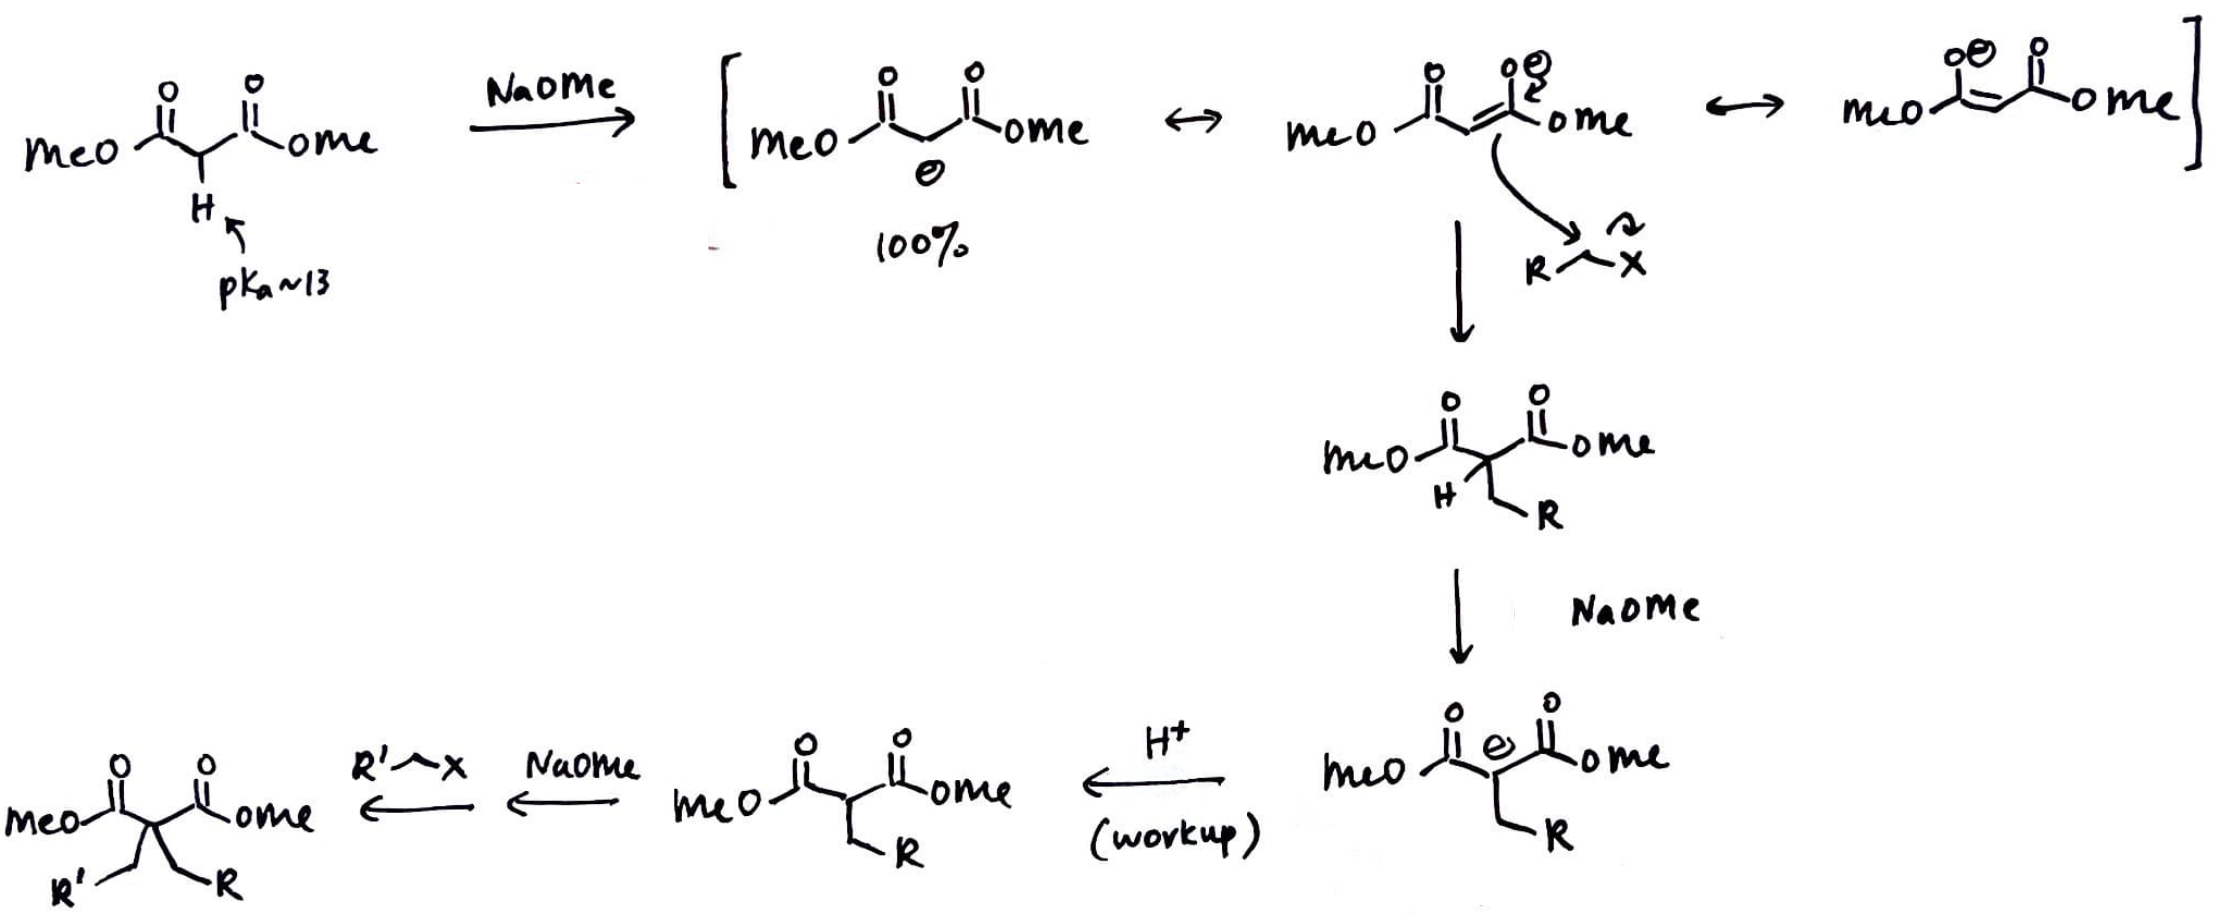
\includegraphics[width=0.9\linewidth]{malEsterSynth.png}
        \caption{Malonate ester synthesis.}
        \label{fig:malEsterSynth}
    \end{figure}
    \pagebreak
    \begin{itemize}
        \item Recall malonate esters from last class (see Figure \ref{fig:alphaAlkMalEstera}).
        \item Since these compounds have $\pKa\approx 13$ at their $\alpha$-protons, \ce{NaOMe} can do 100\% deprotonation.
        \begin{itemize}
            \item Note that we match the base to the ester: Dimethyl malonate should be paired with \ce{NaOMe} in \ce{MeOH} and diethyl malonate should be paired with \ce{NaOEt} in \ce{EtOH}.
            \item This is because we'll have competitive transesterification (see Figure \ref{fig:transesterBase}), so matching the base ensures that we don't get a mixture of products.
        \end{itemize}
        \item Our deprotonated malonate ester can then attack some \ce{C-X} bond, alkylating the $\alpha$-position.
        \item But we're still in basic solution, so our species will be deprotonated until water workup.
        \begin{itemize}
            \item Do assume that we will \emph{not} get competitive dialkylation.
            \item However, alternatively, we could add more base and another \ce{C-X} species to yield a dialkylated species.
        \end{itemize}
        \item These reactions are collectively known as the \textbf{malonate ester synthesis}.
    \end{itemize}
    \item TTQ: Given propane-1,3-diol, \ce{MeI}, and \ce{EtI}, make the product shown in Figure ??a.
    \begin{figure}[h!]
        \centering
        \begin{subfigure}[b]{\linewidth}
            \centering
            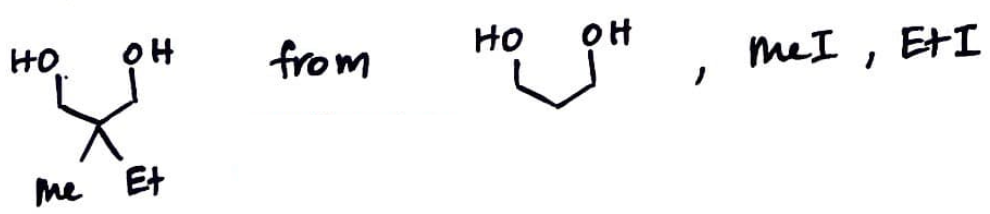
\includegraphics[width=0.4\linewidth]{TTQalpha13diola.png}
            \caption{The desired molecule and starting materials.}
            \label{fig:TTQalpha13diola}
        \end{subfigure}\\[2em]
        \begin{subfigure}[b]{\linewidth}
            \centering
            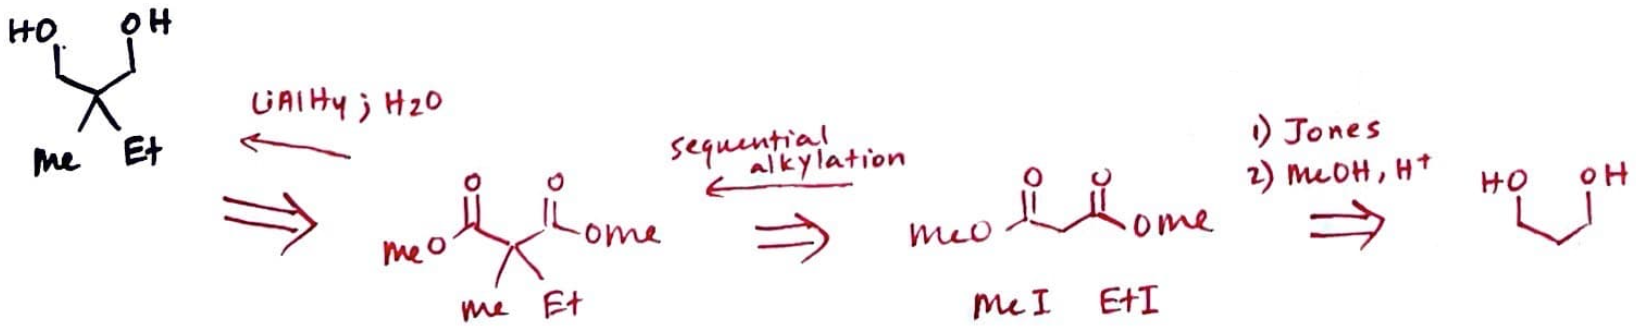
\includegraphics[width=0.65\linewidth]{TTQalpha13diolb.png}
            \caption{Retrosynthetic pathway.}
            \label{fig:TTQalpha13diolb}
        \end{subfigure}
        \caption{TTQ: Synthesis of an $\alpha$-substituted 1,3-diol.}
        \label{fig:TTQalpha13diol}
    \end{figure}
    \begin{itemize}
        \item You might get greedy and start thinking about how to deprotonate the middle carbon directly, but we can't do that; we have to go back to something more reasonable first.
        \item Indeed, we can do a malonate ester synthesis with sequential alkylations followed by LAH reduction to the diol!
        \item Tip: Whenever you see a 1,3-diol, you should ask yourself if a malonate ester can be used!
        \item Note that we make the malonate ester from the 1,3-diol via Jones oxidation (see Figure \ref{fig:OxAlcAlda}) followed by Fischer esterification (see Figure \ref{fig:acylTFischer}).
    \end{itemize}
    \item We now discuss a related process called the \textbf{acetoacetate synthesis}.
    \begin{figure}[h!]
        \centering
        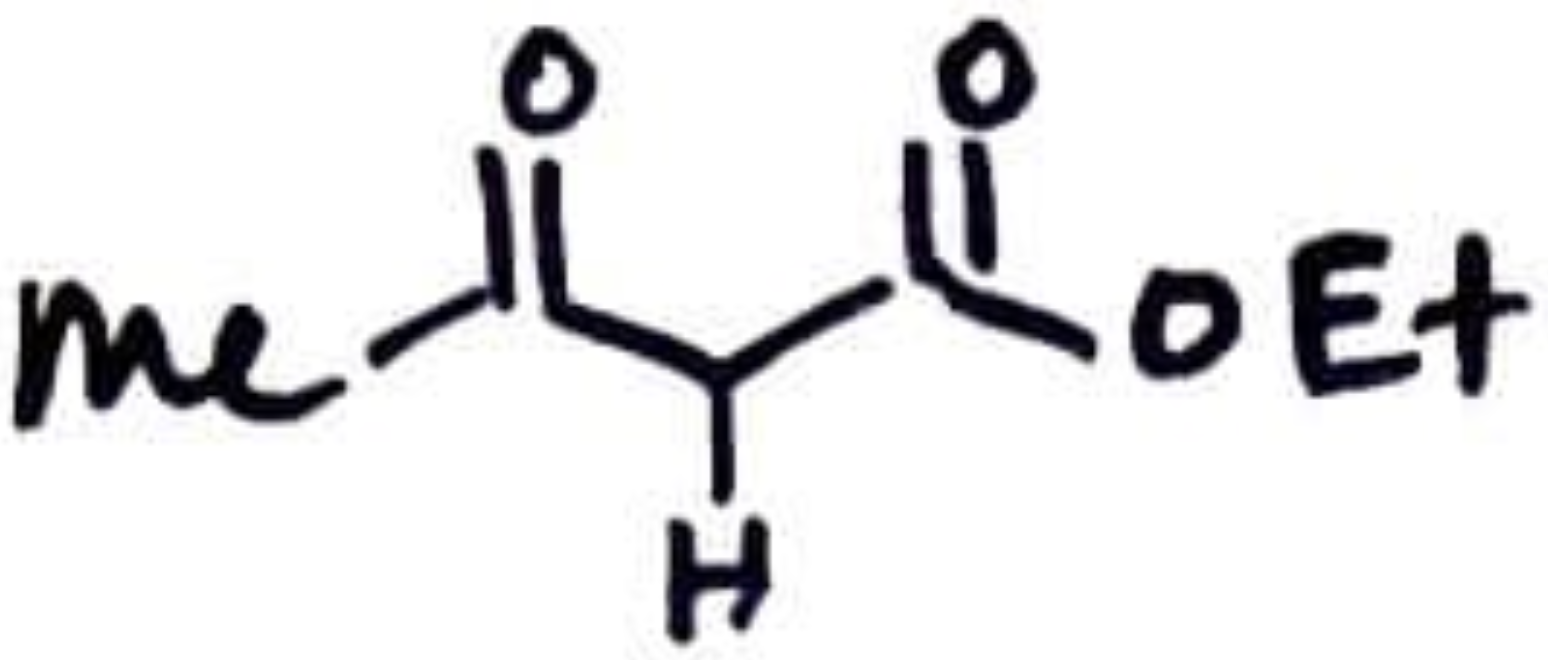
\includegraphics[width=0.15\linewidth]{EtOacac.png}
        \caption{Ethyl acetoacetate.}
        \label{fig:EtOacac}
    \end{figure}
    \begin{itemize}
        \item Here, we have a \emph{ketone} next to an ester group.
        \begin{itemize}
            \item The reason that one is an ethyl ester and the other is a methyl ester is historical; we are totally fine to use ethyl or methyl esters wherever, as long as we're consistent.
        \end{itemize}
        \item $\pKa\approx 11$ for ethyl acetoacetate.
    \end{itemize}
    \item Let's now begin the synthesis.
    \begin{figure}[H]
        \centering
        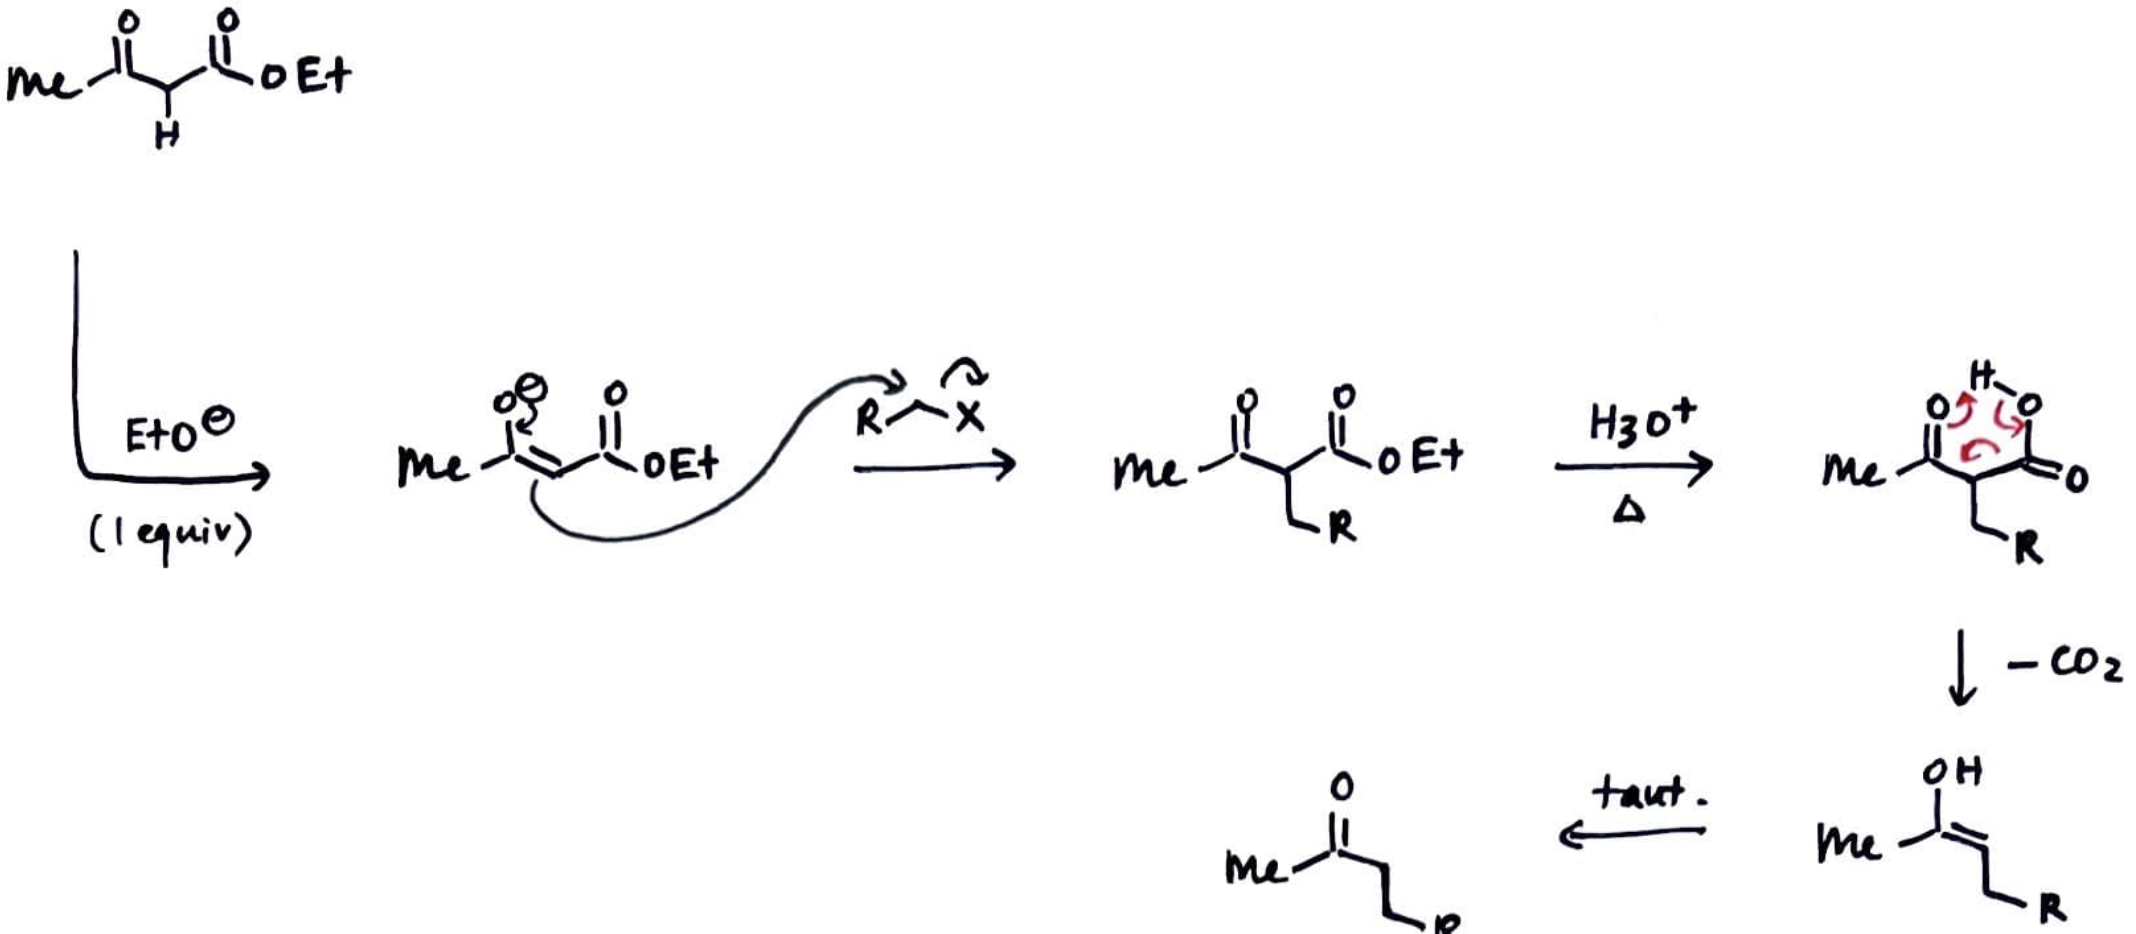
\includegraphics[width=0.9\linewidth]{acacSynth.png}
        \caption{Acetoacetate synthesis.}
        \label{fig:acacSynth}
    \end{figure}
    \begin{itemize}
        \item Adding 1 equivalent of \ce{EtO-} deprotonates to the enolate.
        \begin{itemize}
            \item Note that the resonance will be primarily with the ketone, \emph{not} the ester!
        \end{itemize}
        \item Then we can do our alkylation.
        \begin{itemize}
            \item We could even do a second alkylation, but we're just not going to show that here.
        \end{itemize}
        \item Next step: We heat our intermediate in acid, which first gives ester hydrolysis to the \textbf{$\bm{\beta}$-ketoacid}.
        \begin{itemize}
            \item $\beta$-ketoacids are known to undergo decarboxylation to yield enols!
        \end{itemize}
        \item However, in acidic solution, our enol will quickly tautomerize to a ketone.
        \item Takeaway: This reaction is equivalent to enolate alkylation with LDA (see Figure \ref{fig:enolateKinetic}).
        \begin{itemize}
            \item However, LDA is pyrophoric and hence nasty to work with.
            \item The acetoacetate synthesis, however, is \textbf{bucket chemistry} (easy, safe, and scalable).
        \end{itemize}
    \end{itemize}
    \item TTQ: Make 2-methylhexa-1,5-diene from ethyl acetoacetate, allyl bromide, any other reagent we want with two or fewer carbons, and any other non-carbon reagent.
    \begin{figure}[H]
        \centering
        \begin{subfigure}[b]{\linewidth}
            \centering
            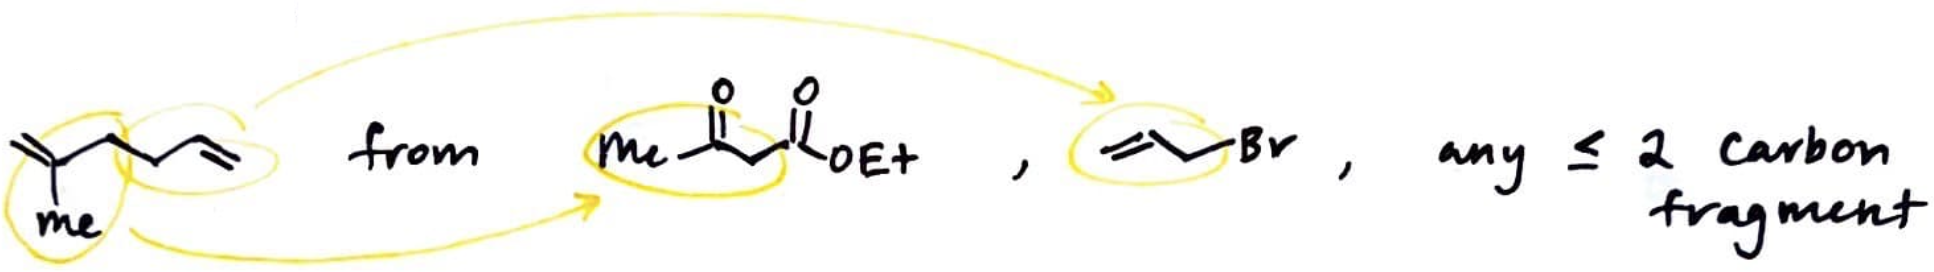
\includegraphics[width=0.75\linewidth]{TTQacaca.png}
            \caption{The desired molecule and starting materials.}
            \label{fig:TTQacaca}
        \end{subfigure}\\[1em]
        \begin{subfigure}[b]{\linewidth}
            \centering
            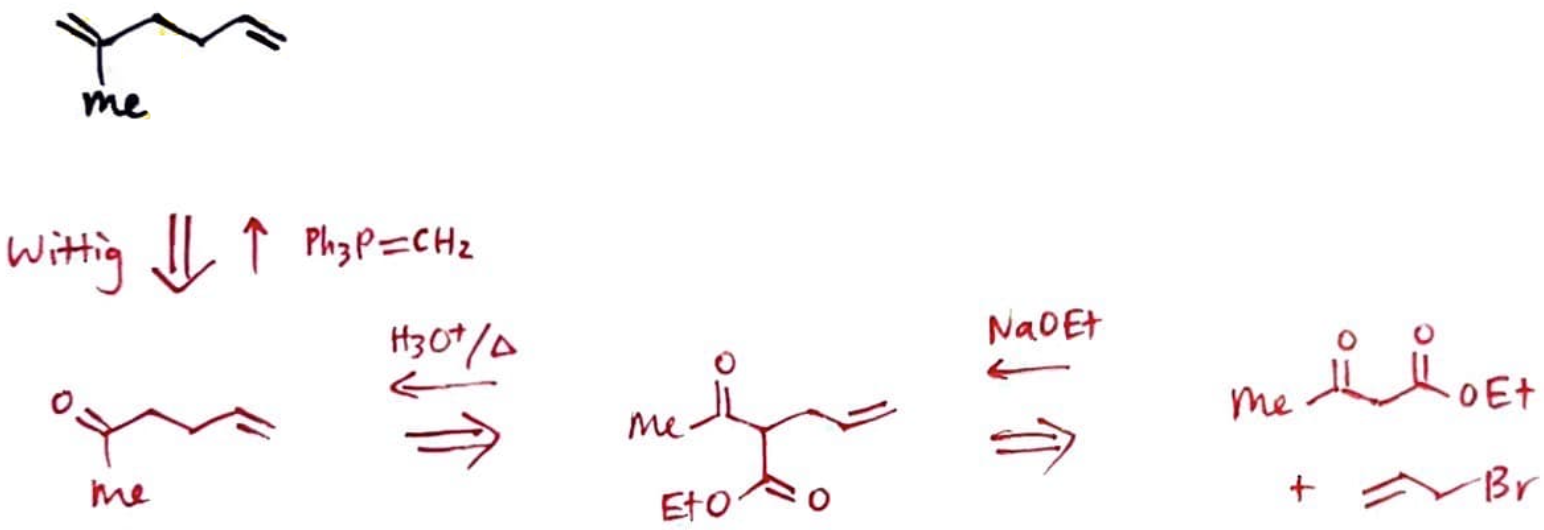
\includegraphics[width=0.65\linewidth]{TTQacacb.png}
            \caption{Retrosynthetic pathway.}
            \label{fig:TTQacacb}
        \end{subfigure}
        \caption{TTQ: Using the acetoacetate synthesis.}
        \label{fig:TTQacac}
    \end{figure}
    \begin{itemize}
        \item Match up the carbons as we've done previously.
        \item A Wittig would yield the product.
        \item Next step: We can go back to the acetoacetate.
        \item Next step: Do alkylation from the starting materials.
    \end{itemize}
\end{itemize}



\section{Aldol Reactions}
\begin{itemize}
    \item \marginnote{11/20:}Announcements.
    \begin{itemize}
        \item PSet 7 is due before Thanksgiving so that you don't have to spend the break thinking about it! However, you should feel free to turn it in the Saturday of Thanksgiving by noon if it's too hard to get it in before the break.
        \item On PSets and exams, please only use reactions covered in 5.12 and 5.13!! Using knowledge from your research only makes grading more difficult for the TFs, and will not score you any more points.
        \item The practice exams for Exam 4 will go up next Monday.
        \begin{itemize}
            \item They will \emph{not} cover material that hasn't been covered in class this time around.
        \end{itemize}
    \end{itemize}
    \item Lecture 30 recap.
    \begin{itemize}
        \item Prof. Buchwald redraws Table \ref{tab:enolateBase}, Figure \ref{fig:enolateKinetic}, and Figure \ref{fig:enolateThermodynamic}.
        \begin{itemize}
            \item Note that whenever we use LDA, we need \emph{at least} 1 equivalent of it to ensure irreversibility.
        \end{itemize}
        \item Good enolate alkylating agent include primary alkyl, methyl, benzyl, and allyl groups.
        \begin{itemize}
            \item $\ce{X}=\ce{Br},\ce{I},\ce{OTs}$.
            \item There are other alkylating agents, but we're just not discussing them.
        \end{itemize}
        \item $\beta$-dicarbonyl species are called "soft enolates," because they do less competitive chemistry.
    \end{itemize}
    \item Today: Aldol reactions.
    \begin{itemize}
        \item Etymology: \underline{Ald}ehyde starting material and alcoh\underline{ol} product.
        \item We'll discuss more named reactions later on this semester (Diekmann, Michael, Claisen), but this one is not named after a person.
    \end{itemize}
    \item Lecture outline.
    \begin{enumerate}[label={\Alph*.},start=4]
        \item Aldol reactions.
        \begin{itemize}
            \item General form.
            \item Acid-catalyzed mechanism.
            \item Base-catalyzed mechanism.
            \item Dehydration of aldol adducts.
            \item Complications.
        \end{itemize}
    \end{enumerate}
    \item General form.
    \begin{figure}[h!]
        \centering
        \footnotesize
        \schemestart
            \chemname{
                \chemfig{Me-[:30](=[2]O)-[:-30]Me}
            }{\color{white}$\beta$}
            \arrow{0}[,0.1]\+{,,1.1em}
            \chemname{
                \chemfig{Me-[:30](=[2]O)-[:-30]Me}
            }{\color{white}$\beta$}
            \arrow{<=>[cat]}[,1.3]
            \chemname{
                \chemfig{Me-[:30](=[2]O)-[:-30]-[:30](-[2]OH)(-[:-70]Me)-[:-30]Me}
            }{$\beta$-hydroxyketone}
            \arrow{->[cat \ce{H+}][or \ce{HO-}]}[,1.3]
            \chemname{
                \chemfig{Me-[:30](=[2]O)-[:-30]=_[:30](-[2]Me)-[:-30]Me}
            }{$\alpha,\beta$-unsaturated ketone}
        \schemestop
        \caption{Aldol condensation.}
        \label{fig:aldol}
    \end{figure}
    \begin{itemize}
        \item The catalyst is typically an acid or base.
        \item The first step is a condensation, and the second is a dehydration.
        \item Tip: If we see a $\beta$-hydroxyaldehyde or $\beta$-hydroxyketone in a synthesis question, think aldol!
        \begin{itemize}
            \item If you see an $\alpha,\beta$-unsaturated carbonyl, you should also think aldol.
        \end{itemize}
    \end{itemize}
    \item Review: How does the ketone appear in acidic solution? It exists in a few forms.
    \begin{figure}[h!]
        \centering
        \vspace{0.5em}
        \footnotesize
        \schemestart
            \chemfig{Me-[:30](=[2]\charge{135=$\oplus$}{O}H)-[:-30]Me}
            \arrow{<->>}
            \chemfig{Me-[:30](=[2]O)-[:-30]Me}
            \arrow{<<->}
            \chemfig{Me-[:30](-[2]OH)=_[:-30]}
        \schemestop
        \caption{Forms of a ketone in acidic media.}
        \label{fig:ketoneFormAcid}
    \end{figure}
    \begin{itemize}
        \item The majority is as the ketone.
        \item It can also be protonated.
        \begin{itemize}
            \item This protonated species is a great electrophile, but there's only a little bit of it.
            \item It is in equilibrium with the regular ketone.
        \end{itemize}
        \item The ketone can also form the enol in very small amount.
        \begin{itemize}
            \item This is a moderate nucleophile.
        \end{itemize}
        \item Recall that there is \emph{no} enolate in acidic media!
    \end{itemize}
    \item Acid-catalyzed mechanism.
    \begin{figure}[h!]
        \centering
        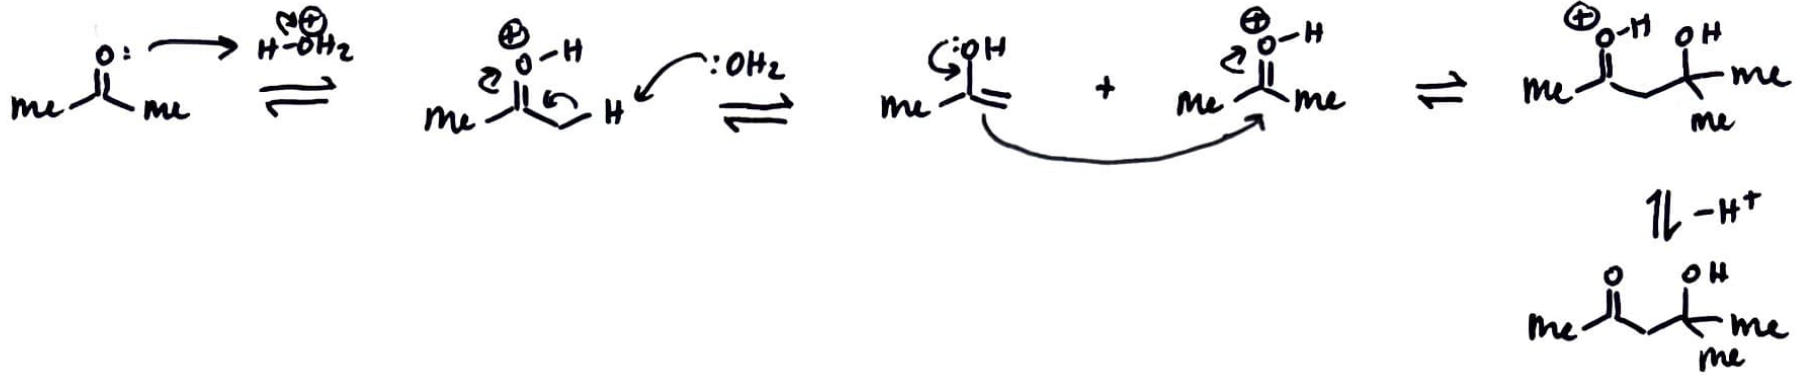
\includegraphics[width=\linewidth]{aldolMechAcid.png}
        \caption{Aldol reaction mechanism (acid-catalyzed).}
        \label{fig:aldolMechAcid}
    \end{figure}
    \begin{itemize}
        \item In the first step of the mechanism, we protonate the ketone to its protonated form.
        \item We then deprotonate at the $\alpha$-position to form the enol.
        \item The enol can then nucleophilically attack another molecule of protonated ketone.
        \item Finally, we deprotonated to the aldol.
        \item Important note: Every step is reversible!
    \end{itemize}
    \item Review: How does the ketone appear in basic solution? It also exists in a few forms.
    \begin{figure}[h!]
        \centering
        \vspace{0.5em}
        \footnotesize
        \schemestart
            \chemfig{Me-[:30](=[2]O)-[:-30]Me}
            \arrow{<<->}
            \chemfig{Me-[:30](=[2]\charge{45=$\ominus$}{O})-[:-30]Me}
            \arrow{<=>}
            \chemfig{Me-[:30](-[2]OH)=_[:-30]}
        \schemestop
        \caption{Forms of a ketone in basic media.}
        \label{fig:ketoneFormBase}
    \end{figure}
    \pagebreak
    \begin{itemize}
        \item The majority is as the ketone, once again.
        \item It can exist as the enolate.
        \begin{itemize}
            \item This species is a great nucleophile, but there's only a little bit of it.
        \end{itemize}
        \item The ketone can also form the enol in very small amount.
        \begin{itemize}
            \item This is a moderate nucleophile.
        \end{itemize}
        \item Recall that there is \emph{no} protonated ketone in basic media!
    \end{itemize}
    \item Base-catalyzed mechanism.
    \begin{figure}[h!]
        \centering
        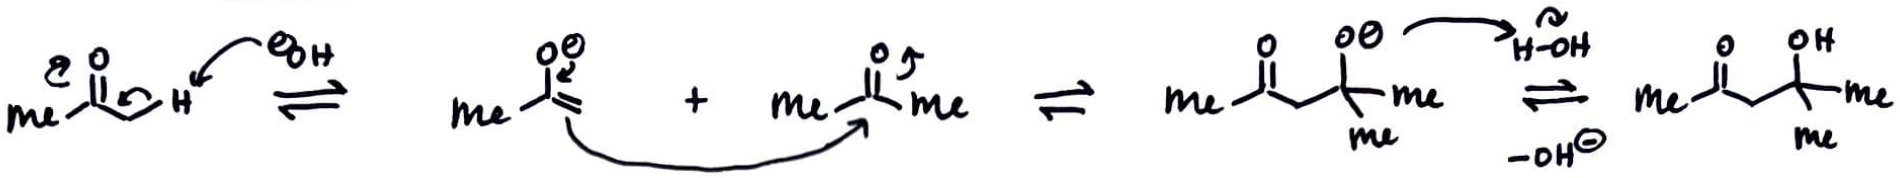
\includegraphics[width=\linewidth]{aldolMechBase.png}
        \caption{Aldol reaction mechanism (base-catalyzed).}
        \label{fig:aldolMechBase}
    \end{figure}
    \begin{itemize}
        \item In the first step of the mechanism, hydroxide comes in to form the enolate.
        \item The enolate then adds nucleophilically into a molecule of (regular, nonprotonated) ketone.
        \item We then protonated the oxyanion to form the aldol.
        \item Important note: Every step is reversible, once again!
        \item This is a very efficient process: Base-catalyzed, with no cationic intermediates.
    \end{itemize}
    \item How do we get from the aldol adduct to the $\alpha,\beta$-unsaturated ketone?
    \item Via the \textbf{dehydration} of aldol adducts!
    \item \textbf{Dehydration} (reaction): A reaction that involves the loss of \ce{H2O}.
    \item A possible (but incorrect!) acidic mechanism.
    \begin{figure}[h!]
        \centering
        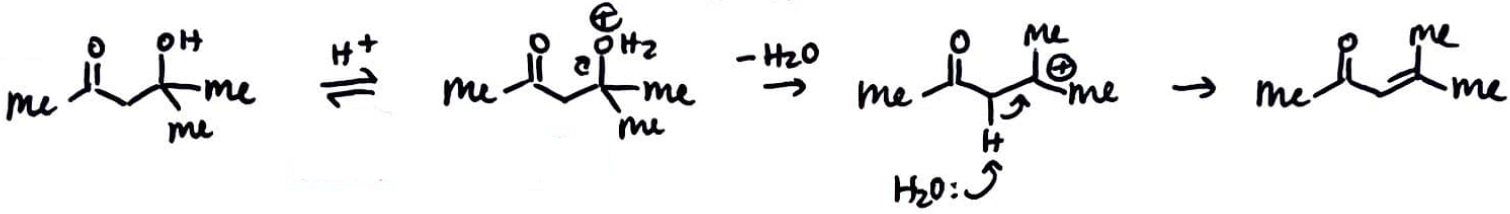
\includegraphics[width=0.85\linewidth]{aldolDehMechAcidInc.png}
        \caption{Incorrect acid-cataylzed aldol dehydration mechanism.}
        \label{fig:aldolDehMechAcidInc}
    \end{figure}
    \begin{itemize}
        \item In acidic media, we protonate the alcohol, which then leaves to give a tertiary carbocation.
        \item Tertiary carbocations are ok here because we have all that hyperconjugation stabilization.
        \item Then we get subsequent elimination to the $\alpha,\beta$-unsaturated ketone product.
    \end{itemize}
    \item To understand the real mechanism, consider the tetrahedral intermediates.
    \begin{figure}[h!]
        \centering
        \begin{subfigure}[b]{0.37\linewidth}
            \centering
            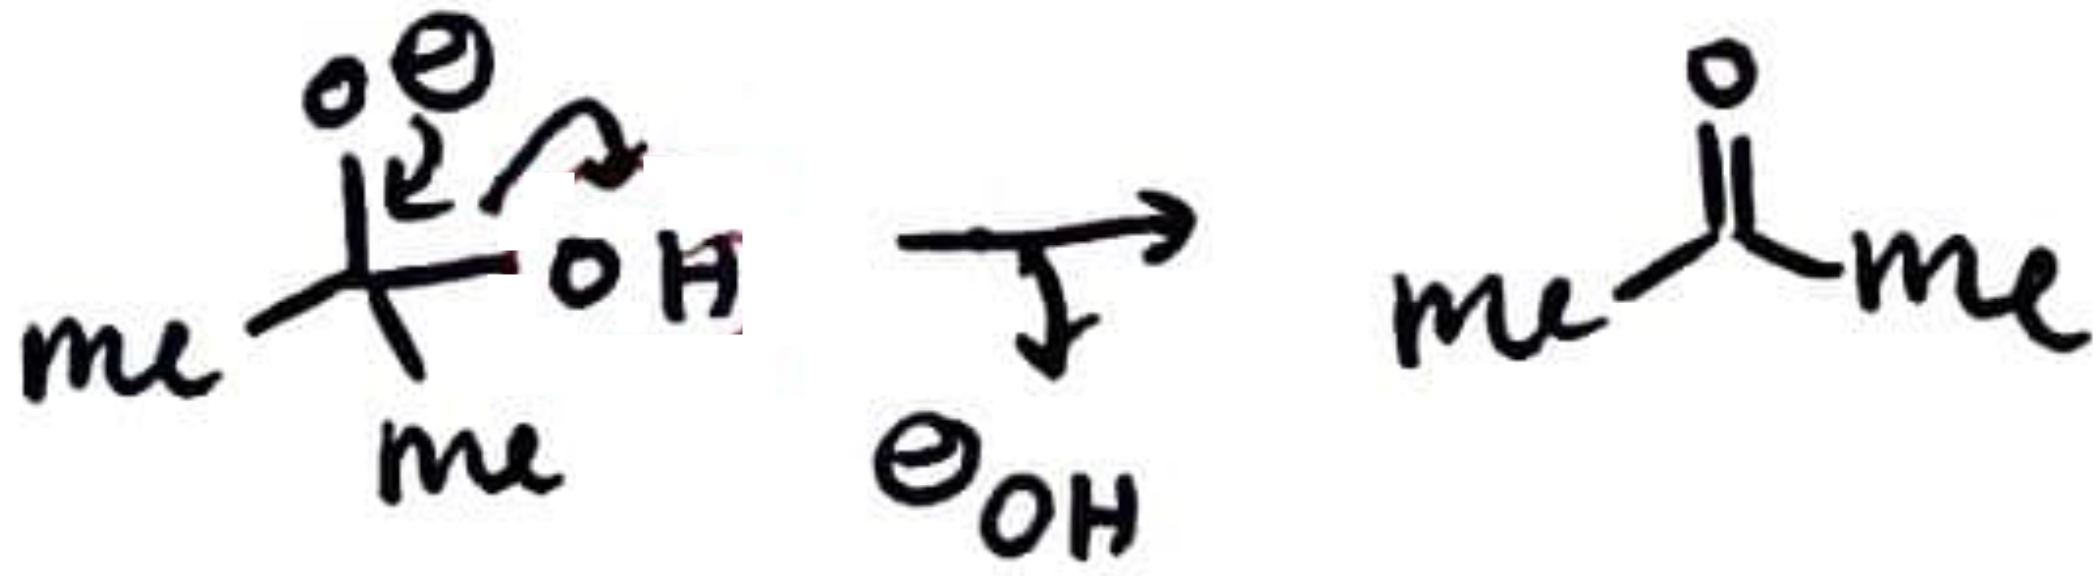
\includegraphics[width=0.8\linewidth]{pushGroupa.png}
            \caption{Pushing hydroxide.}
            \label{fig:pushGroupa}
        \end{subfigure}
        \begin{subfigure}[b]{0.37\linewidth}
            \centering
            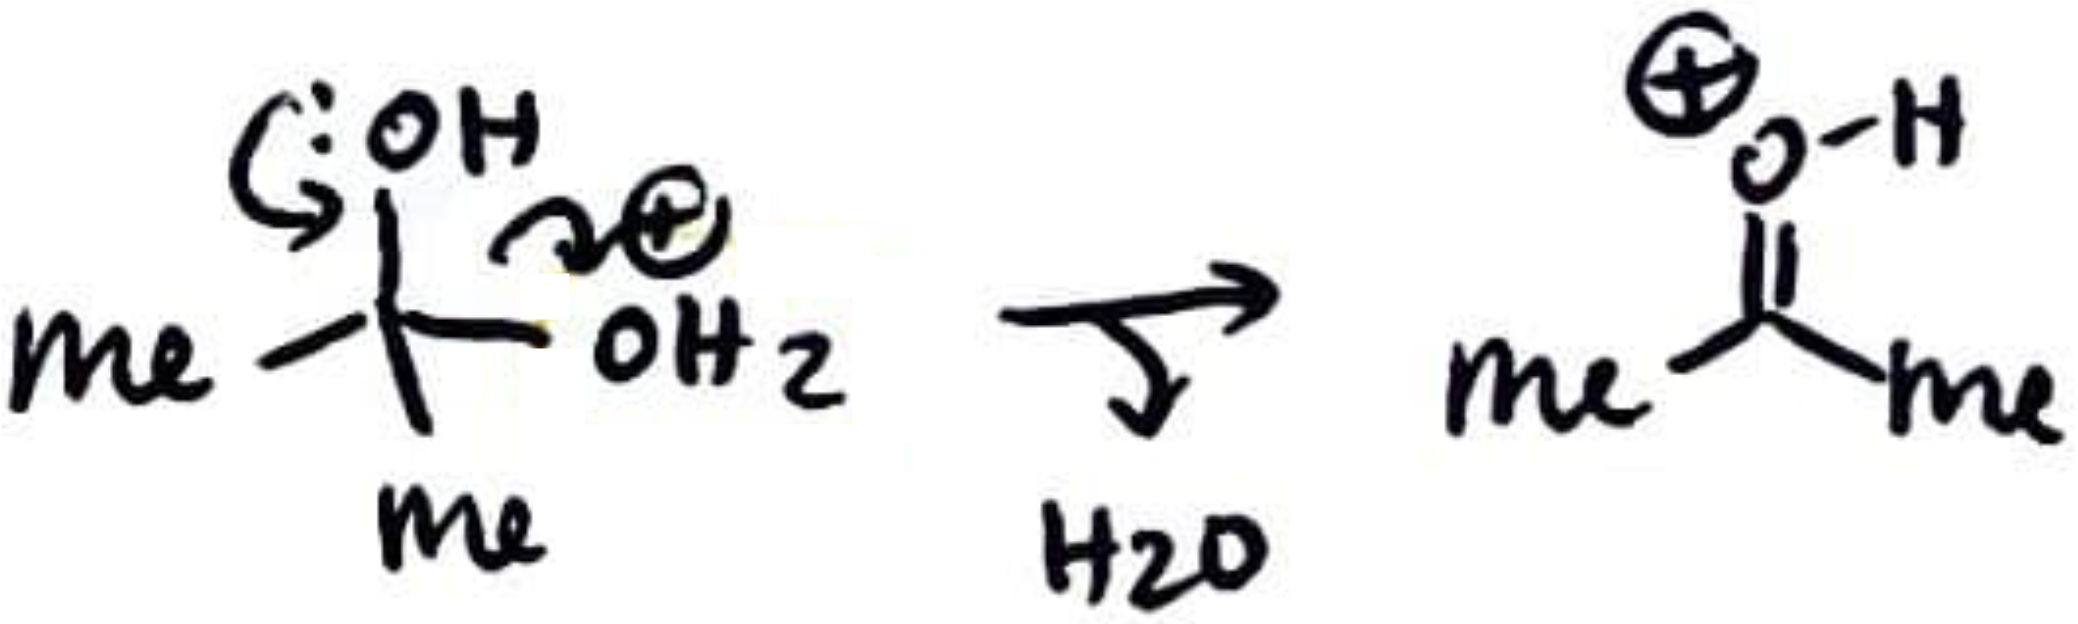
\includegraphics[width=0.8\linewidth]{pushGroupb.png}
            \caption{Pushing water.}
            \label{fig:pushGroupb}
        \end{subfigure}
        \caption{Push groups in tetrahedral intermediates.}
        \label{fig:pushGroup}
    \end{figure}
    \begin{itemize}
        \item Hydroxide is a bad leaving group, but if we have a \textbf{push group} (ideally an anionic species) in the tetrahedral intermediate, we can kick it out (Figure \ref{fig:pushGroupa}).
        \item In acidic media, \ce{OH} is typically not that good of a push group, but it is able to push out water, which can then come back and remove the proton (Figure \ref{fig:pushGroupb}).
    \end{itemize}
    \item In aldol reactions, alkenes act as "electron conduits."
    \begin{figure}[h!]
        \centering
        \begin{subfigure}[b]{0.37\linewidth}
            \centering
            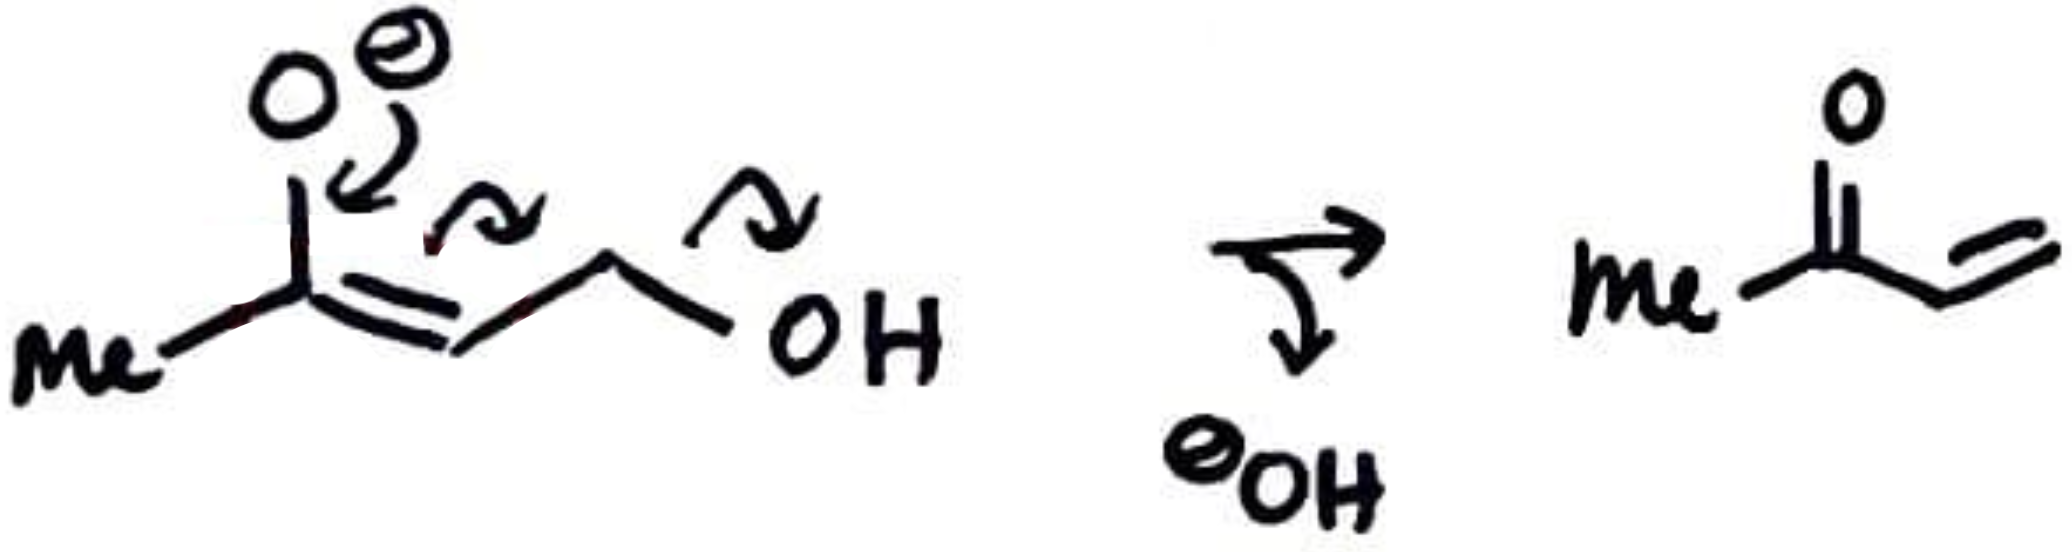
\includegraphics[width=0.88\linewidth]{pushGroupDistanta.png}
            \caption{Pushing hydroxide.}
            \label{fig:pushGroupDistanta}
        \end{subfigure}
        \begin{subfigure}[b]{0.37\linewidth}
            \centering
            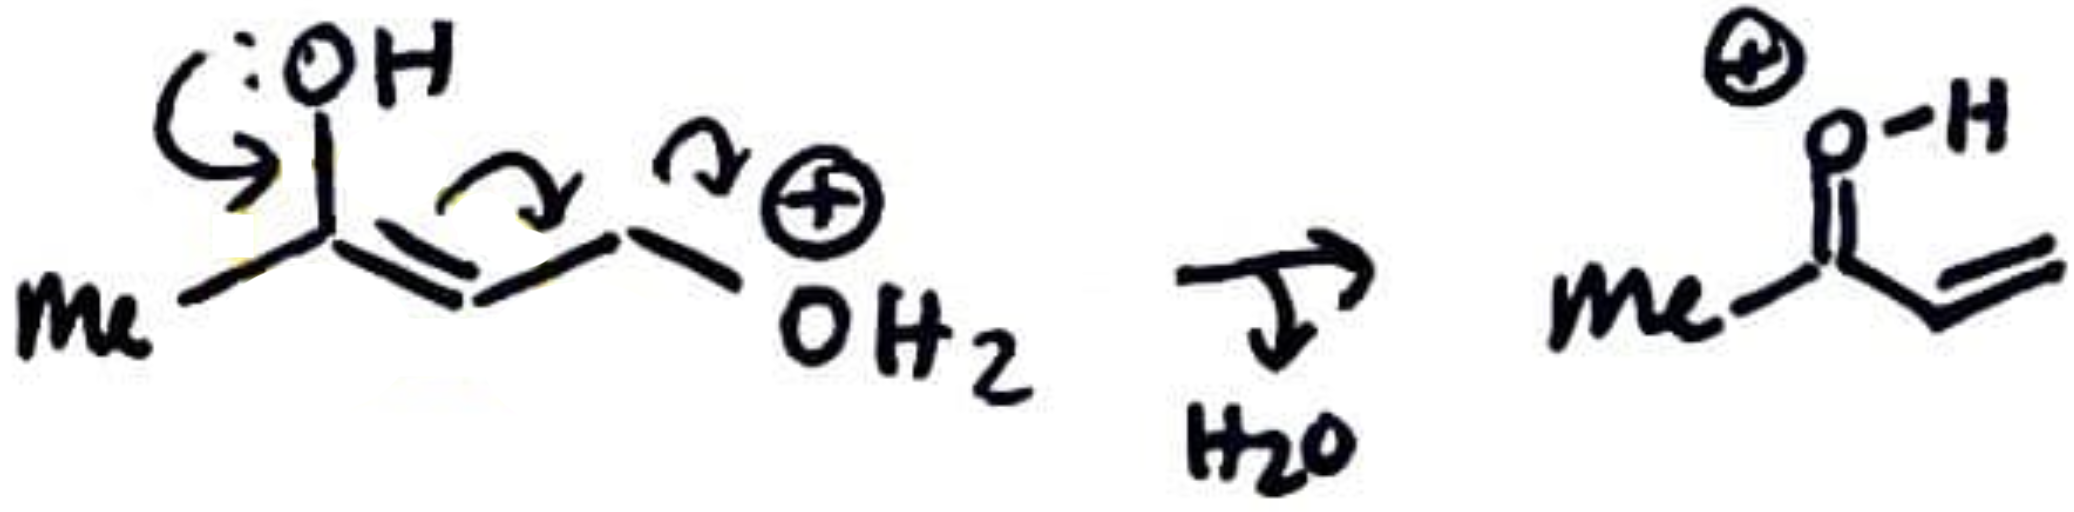
\includegraphics[width=0.88\linewidth]{pushGroupDistantb.png}
            \caption{Pushing water.}
            \label{fig:pushGroupDistantb}
        \end{subfigure}
        \caption{Push groups can act from distant positions through electron conduits.}
        \label{fig:pushGroupDistant}
    \end{figure}
    \begin{itemize}
        \item This allows the (protonated or unprotonated) $\beta$-alcohols to feel the effect of the oxyanion or hydroxyl group even from further away!
    \end{itemize}
    \item With push groups in mind, let's now discuss the \emph{correct} acid-catalyzed aldol dehydration mechanism.
    \begin{figure}[h!]
        \centering
        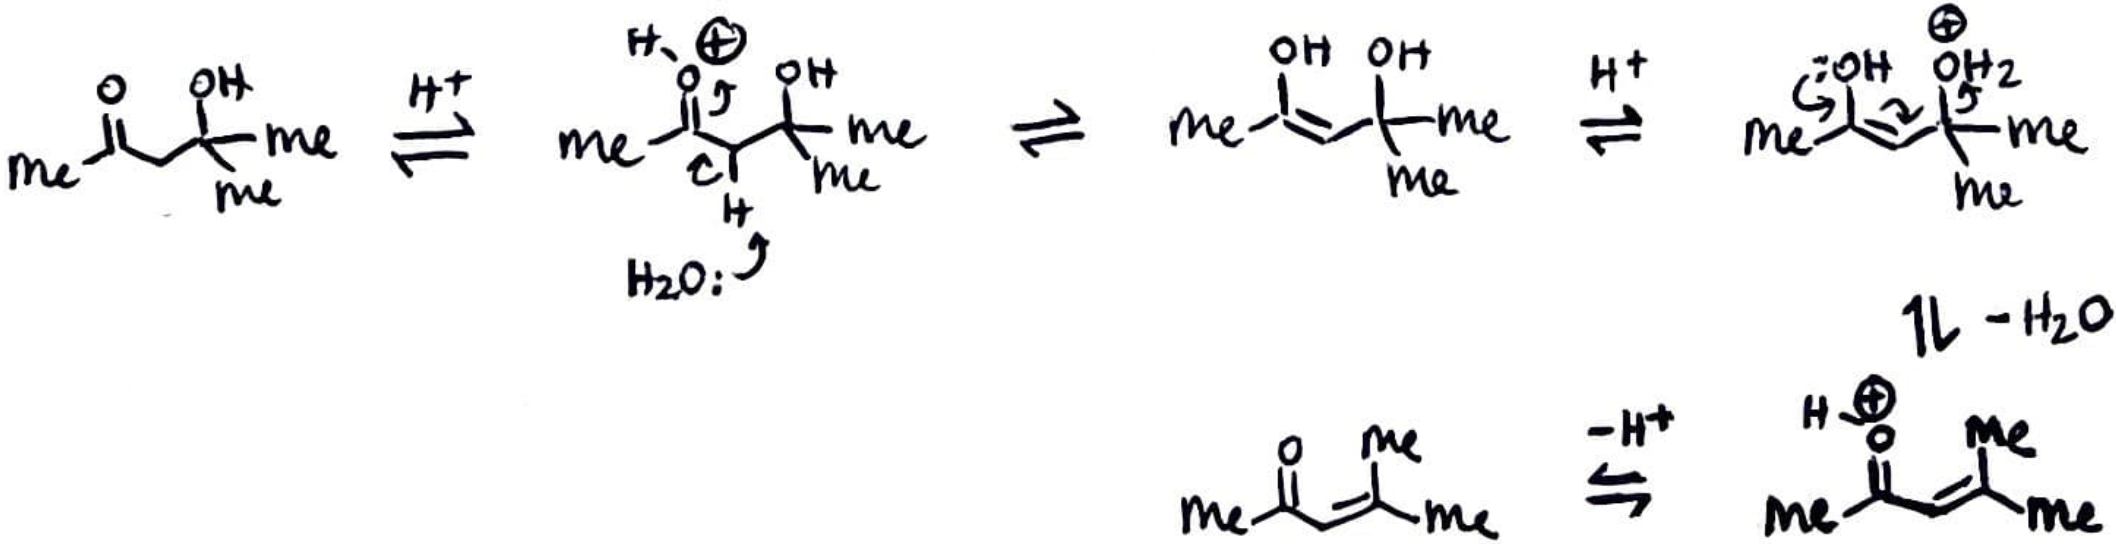
\includegraphics[width=0.9\linewidth]{aldolDehMechAcid.png}
        \caption{Aldol dehydration mechanism (acid-catalyzed).}
        \label{fig:aldolDehMechAcid}
    \end{figure}
    \begin{itemize}
        \item The first two steps are keto-enol tautomerization.
        \item We then protonate the $\beta$-alcohol.
        \item Next, we push it out through out electron conduit.
        \item Finally, we deprotonate our reformed ketone.
    \end{itemize}
    \item To drive these reactions in the forward direction, we often need to remove water.\footnote{Think Le Ch\^{a}telier's principle! Removing one product drives the equilbrium to the right.}
    \begin{itemize}
        \item We can remove water with some kind of dehydrating agent, though we don't need to show this on PSets or exams.
    \end{itemize}
    \item A story from Prof. Buchwald's undergrad years.
    \begin{itemize}
        \item Running a reaction in acetone on a \SI{200}{\milli\gram} scale, but isolated \SI{9}{\gram} of product!
        \item What happened?
        \item Someone had added a dehydrating agent to the bottle of acetone, turning it all into the aldol condensation product! So Prof. Buchwald hadn't used acetone as his solvent; he'd used the above aldol condensation product.
    \end{itemize}
    \item Complications that arise in aldol reactions.
    \pagebreak
    \item Complication \#1: Mixed aldols.
    \begin{figure}[h!]
        \centering
        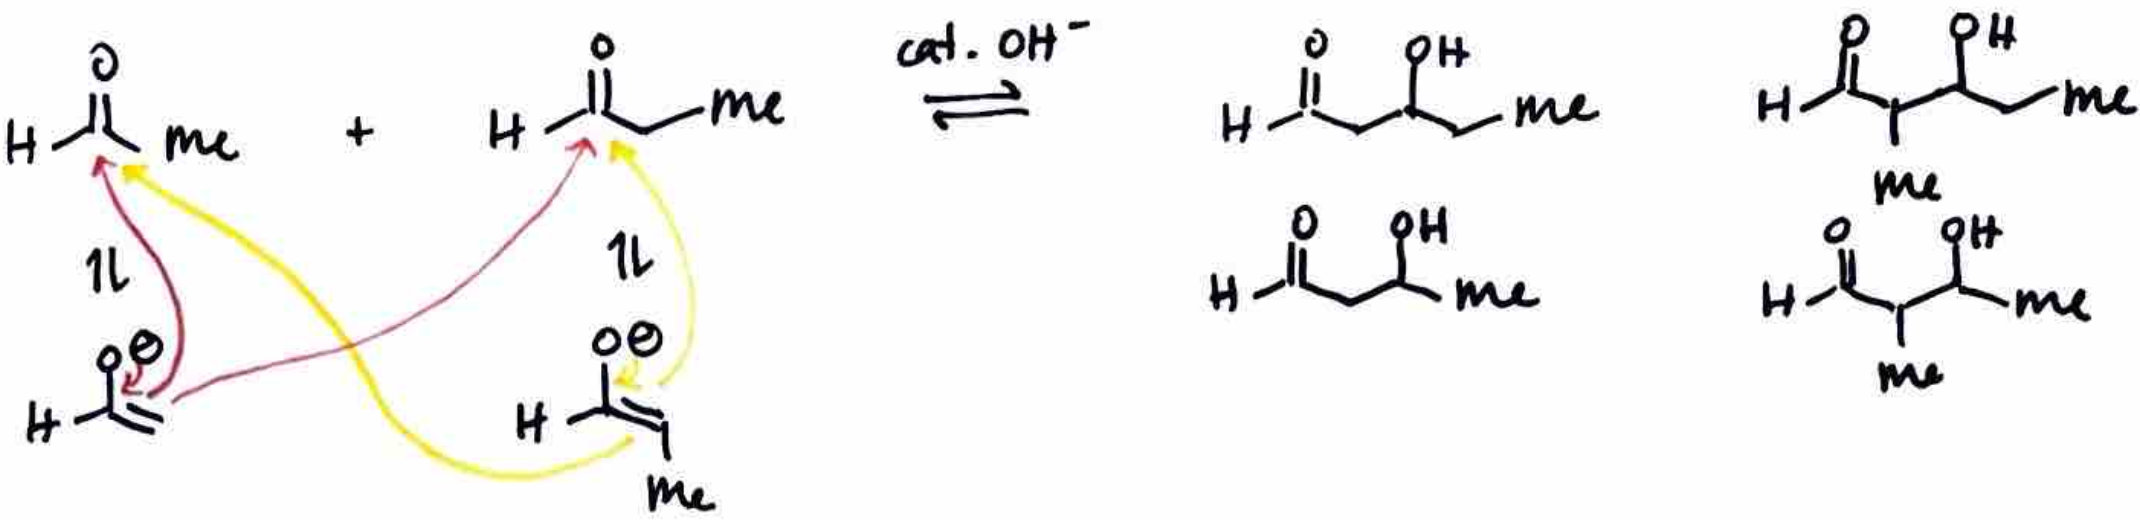
\includegraphics[width=0.85\linewidth]{mixedAldol.png}
        \caption{Mixed aldol reaction product distribution.}
        \label{fig:mixedAldol}
    \end{figure}
    \begin{itemize}
        \item This is what happens if we have two kinds of potential enolate-forming species in solution.
        \item We'll get a mixture of cross-condensation and self-condensation products! There's no way to do this selectively.
        \item And we're all about \emph{efficiency} and \emph{elegance} in 5.13, so we need ways around this.
    \end{itemize}
    \item So how can we pick substrate combinations in which only one component can act as a nucleophile?
    \begin{figure}[h!]
        \centering
        \footnotesize
        \schemestart
            \chemname{
                \chemfig{H-[:30](=[2]O)-[:-30]}
            }{formaldehyde}
            \arrow{0}[,0.7]
            \chemname{
                \chemfig{{}^{\emph{t}}Bu-[:30](=[2]O)-[:-30]}
            }{pivaldehyde}
            \arrow{0}[,0.7]
            \chemname{
                \chemfig{Ph-[:30](=[2]O)-[:-30]}
            }{benzaldehyde}
        \schemestop
        \caption{Non-enolizable carbonyl compound examples.}
        \label{fig:nonEnolizable}
    \end{figure}
    \begin{itemize}
        \item Carbonyls aren't inherently nucleophiles; we make them \emph{into} nucleophiles via deprotonation of an $\alpha$-proton.
        \item But if we make a carbonyl without any $\alpha$-protons, we have a non-enolizable species that can \emph{only} react as an electrophile!
        \item Examples: Formaldehyde, pivaldehyde (smells terrible), and benzaldehyde (smells like almonds).
        \begin{itemize}
            \item Aldehyde protons have high $\pKa$'s and won't be deprotonated.
            \item Note that formaldehyde is a gas, but for the purposes of 5.13, we'll say that we can treat it as a liquid reagent like any other. This isn't entirely false because we can buy liquids that react like they're liquid formaldehyde (i.e., they decompose to formaldehyde \emph{in situ}).
        \end{itemize}
    \end{itemize}
    \item Thus, if we mix acetophenone with formaldehyde, we will only get one aldol product!
    \begin{figure}[h!]
        \centering
        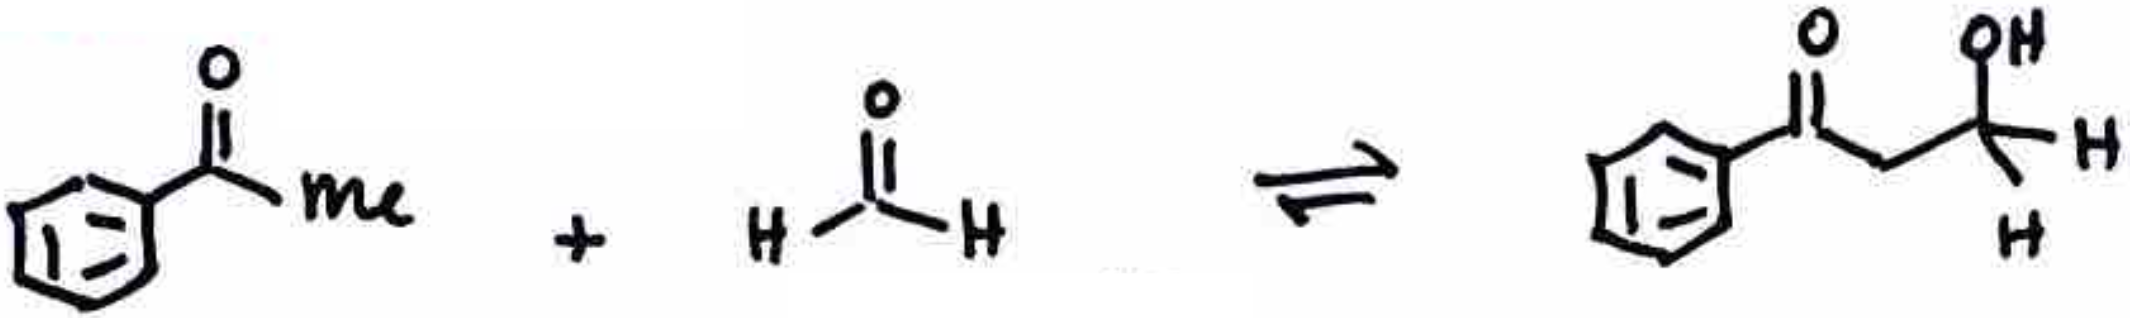
\includegraphics[width=0.6\linewidth]{crossAldolOne.png}
        \caption{Cross-aldol reaction with only one enolizable species.}
        \label{fig:crossAldolOne}
    \end{figure}
    \begin{itemize}
        \item Note that we don't get competitve dimerization of acetophenone because aldehydes are \emph{much} more electrophilic, so they'll react with an enolate \emph{much} faster.
    \end{itemize}
    \pagebreak
    \item Complication \#2: Intramolecular aldol reactions.
    \begin{figure}[h!]
        \centering
        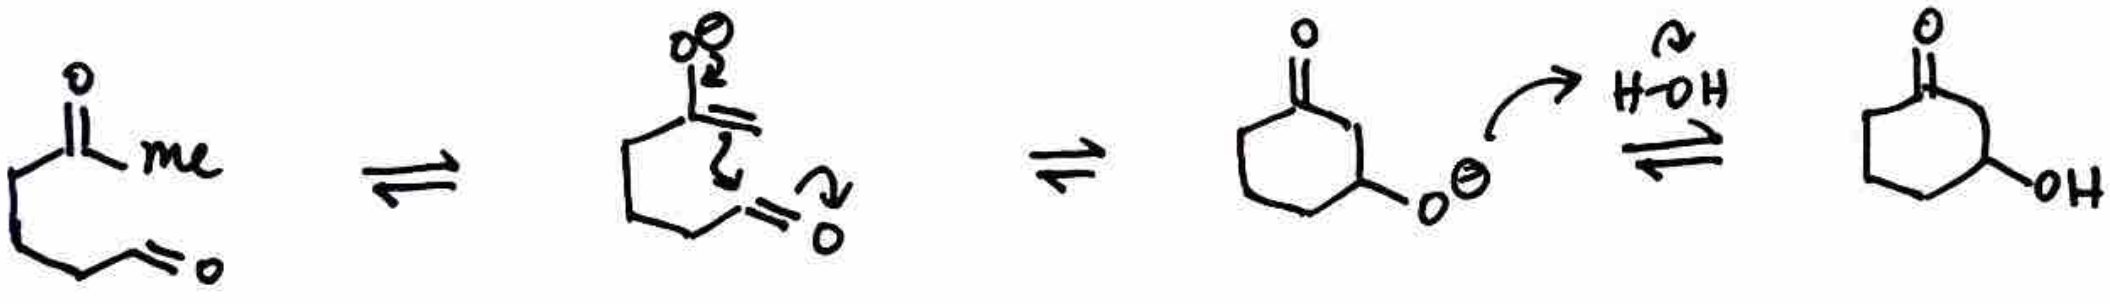
\includegraphics[width=0.8\linewidth]{crossAldolIntra.png}
        \caption{Intramolecular cross-aldol reaction.}
        \label{fig:crossAldolIntra}
    \end{figure}
    \begin{itemize}
        \item Here, we'll form the $\beta$-hydroxy cyclohexanone.
        \item Why did we deprotonate the methyl group? Indeed, we're under equilibrating conditions, so shouldn't we deprotonate at the other side to form the thermodynamic enolate?
        \begin{itemize}
            \item We can form that enolate, but it won't react! The proposed product is a cyclobutane derivative.
            \item Cyclobutanes have \kcal{25} of ring strain.
            \item \kcal{1.4} means 10-fold selectivity, so this cyclobutane product is like 19-orders of magnitude disfavored.
            \item We'll just go from the thermodynamic enolate back to the ketone, until we deprotonate to form the kinetic enolate.
        \end{itemize}
    \end{itemize}
    \item Complication \#3: A modern strategy for cross-aldol reactions between multiple enolizable products.
    \begin{figure}[h!]
        \centering
        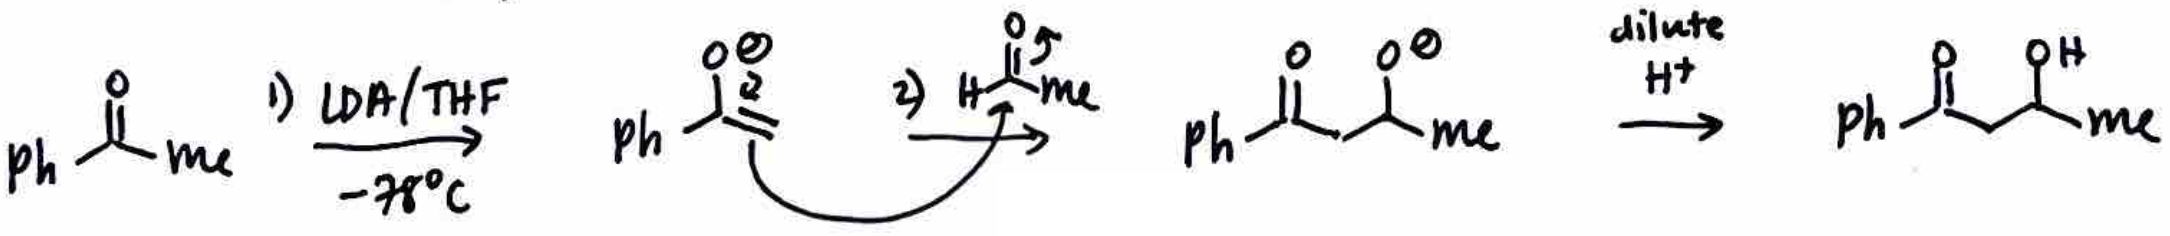
\includegraphics[width=0.9\linewidth]{crossAldolModern.png}
        \caption{Modern cross-aldol reaction.}
        \label{fig:crossAldolModern}
    \end{figure}
    \begin{itemize}
        \item Deprotonate with cold LDA to form the kinetic enolate selectively.
        \item Then add the other coupling partner for quick reactivity.
        \item Note that \emph{p}-\ce{TsOH} is a good acid catalyst for dehydration!
    \end{itemize}
\end{itemize}



\section{Claisen Condensations and Conjugate Additions}
\begin{itemize}
    \item \marginnote{11/22:}Lecture 31 recap.
    \begin{itemize}
        \item Recall Figure \ref{fig:aldol}.
        \begin{itemize}
            \item In an aldol reaction (not the dehydration part), every step is reversible.
        \end{itemize}
        \item Good aldol reactions ar those in which\dots
        \begin{itemize}
            \item Cross-aldols in which only one molecule can enolize;
            \item Self-condensation/dimerization.
            \item Intramolecular;
            \item Use of LDA (1 equivalent) to selectively form the kinetic enolate, then add to an aldehyde.
        \end{itemize}
    \end{itemize}
    \item Lecture outline.
    \begin{enumerate}[label={\Alph*.},start=5]
        \item Claisen condensations.
        \item Michael additions.
        \begin{itemize}
            \item 1,4-additions.
        \end{itemize}
    \end{enumerate}
    \item We'll begin with Topic E: Claisen condensations.
    \begin{itemize}
        \item These were discovered by Ludwig Claisen.
    \end{itemize}
    \item General form.
    \begin{figure}[h!]
        \centering
        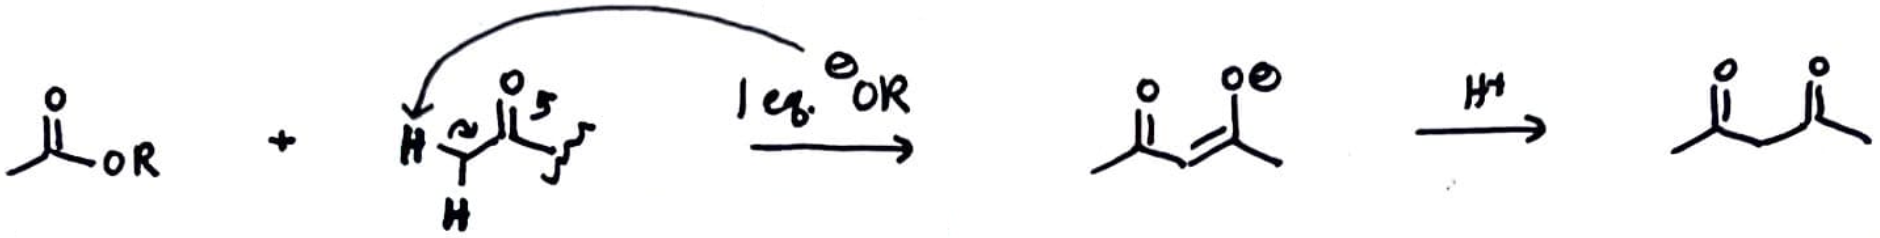
\includegraphics[width=0.85\linewidth]{claisenCondensation.png}
        \caption{Claisen condensation.}
        \label{fig:claisenCondensation}
    \end{figure}
    \begin{itemize}
        \item This is a reaction between an ester and an ester/ketone to form a 1,3-dicarbonyl.
        \item The ester/ketone will become the enolate and attack the other ester.
        \begin{itemize}
            \item It must have at least two protons on its $\alpha$-carbon in order for this reaction to work.
            \item One of these protons will be picked off for the initial condensation, and the second will be picked off to form the enolate drawn above (which is stable until workup).
        \end{itemize}
        \item To prevent (noticeable) transesterification, we use an alkoxide base (\ce{RO-}) matching the ester.
        \item Unlike aldol reactions (see Figure \ref{fig:aldol}), the first step is irreversible here.
        \begin{itemize}
            \item This is because the reaction is driven forward by the formation of a stable enolate in the pre-workup step.
        \end{itemize}
    \end{itemize}
    \item Claisen condensation mechanism.
    \begin{figure}[h!]
        \centering
        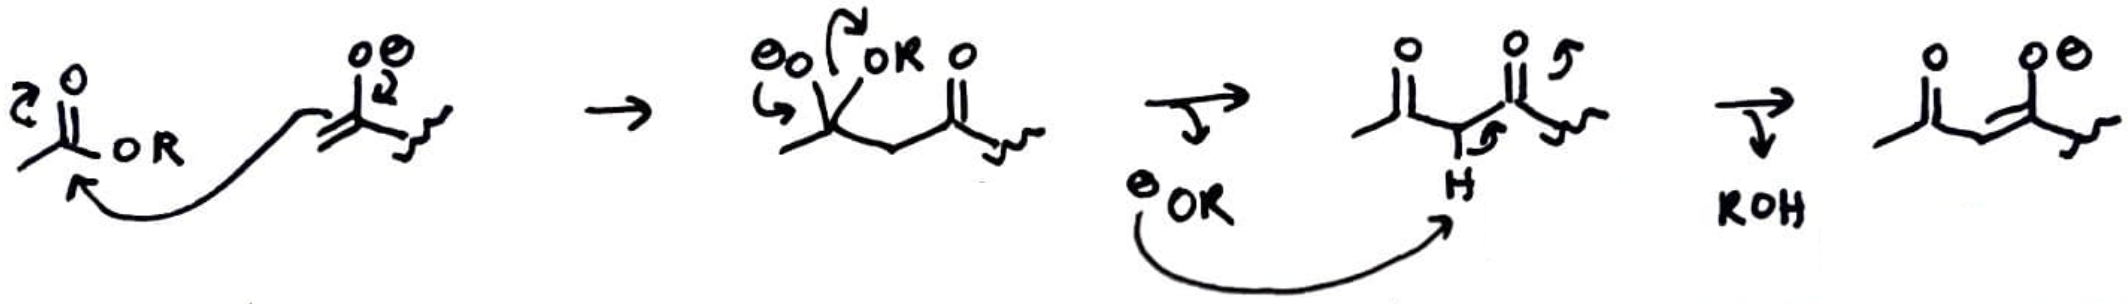
\includegraphics[width=0.9\linewidth]{claisenCondensationMech.png}
        \caption{Claisen condensation mechanism.}
        \label{fig:claisenCondensationMech}
    \end{figure}
    \begin{itemize}
        \item The first step forms a tetrahedral intermediate.
        \item The third step is driven by a $\pKa$ difference: The 1,3-dicarbonyl has $\pKa\approx 9$ and \ce{ROH} has $\pKa\approx 16$, so the alkoxide base will very much favor deprotonating the 1,3-dicarbonyl.
        \item Note again the two different hydrogens that get picked off, and the enolate that is stable until workup.
    \end{itemize}
    \item Under workup conditions, why won't we protonate at the oxygen?
    \begin{itemize}
        \item This would form a $\beta$-ketoenol, and enols are unstable!
        \item Even if we did form this, it would quickly tautomerize to a 1,3-dione.
    \end{itemize}
    \item Self-Claisen condensations.
    \begin{figure}[h!]
        \centering
        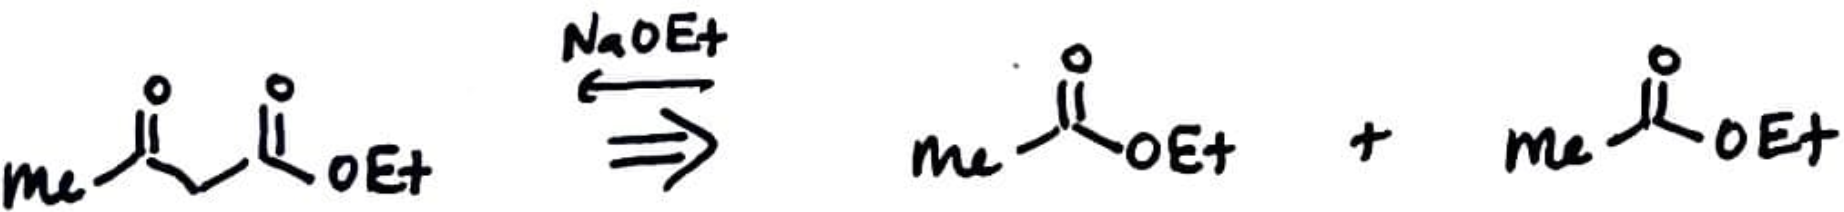
\includegraphics[width=0.6\linewidth]{claisenCondensationSelf.png}
        \caption{Self-Claisen condensations synthesize $\beta$-ketoesters.}
        \label{fig:claisenCondensationSelf}
    \end{figure}
    \begin{itemize}
        \item For the PSet, you will need to be able to make ethyl acetoacetate as above!!
        \item Tip: If you ever need to synthesize a $\beta$-ketoester, think Claisen!
        \item This is especially easy to do if you can start from two equivalents of the same starting material for pseudodimerization, as above.
    \end{itemize}
    \item What about intramolecular Claisen condensations? This is the Dieckmann condensation.
    \begin{itemize}
        \item Walter Dieckmann developed this while in M\"{u}nich at BASF.
    \end{itemize}
    \item General form.
    \begin{figure}[h!]
        \centering
        \footnotesize
        \schemestart
            \chemfig{Me-[:150](=[2,0.6]O)-[:-150,1.3]-[6,1.3]-[:-30,1.3]-[:30,1.3](=[2,0.6]O)-[:-30]OMe}
            \arrow{->[\ce{NaOMe}][\ce{MeOH}]}[,1.3]
            \chemfig{*6(--(=O)--(=O)--)}
        \schemestop
        \caption{Dieckmann condensation.}
        \label{fig:Dieckmann}
    \end{figure}
    \begin{itemize}
        \item As per usual, the solvent is the alcohol that is the conjugate acid of the base used, which in turn is determined by the type of ester used in the starting material.
        \begin{itemize}
            \item For example, here we use \ce{MeOH} and \ce{NaOMe} because our starting material contains a methyl ester.
        \end{itemize}
        \item This reaction can be used to make 5- or 6-membered rings.
    \end{itemize}
    \item Mechanism.
    \begin{figure}[h!]
        \centering
        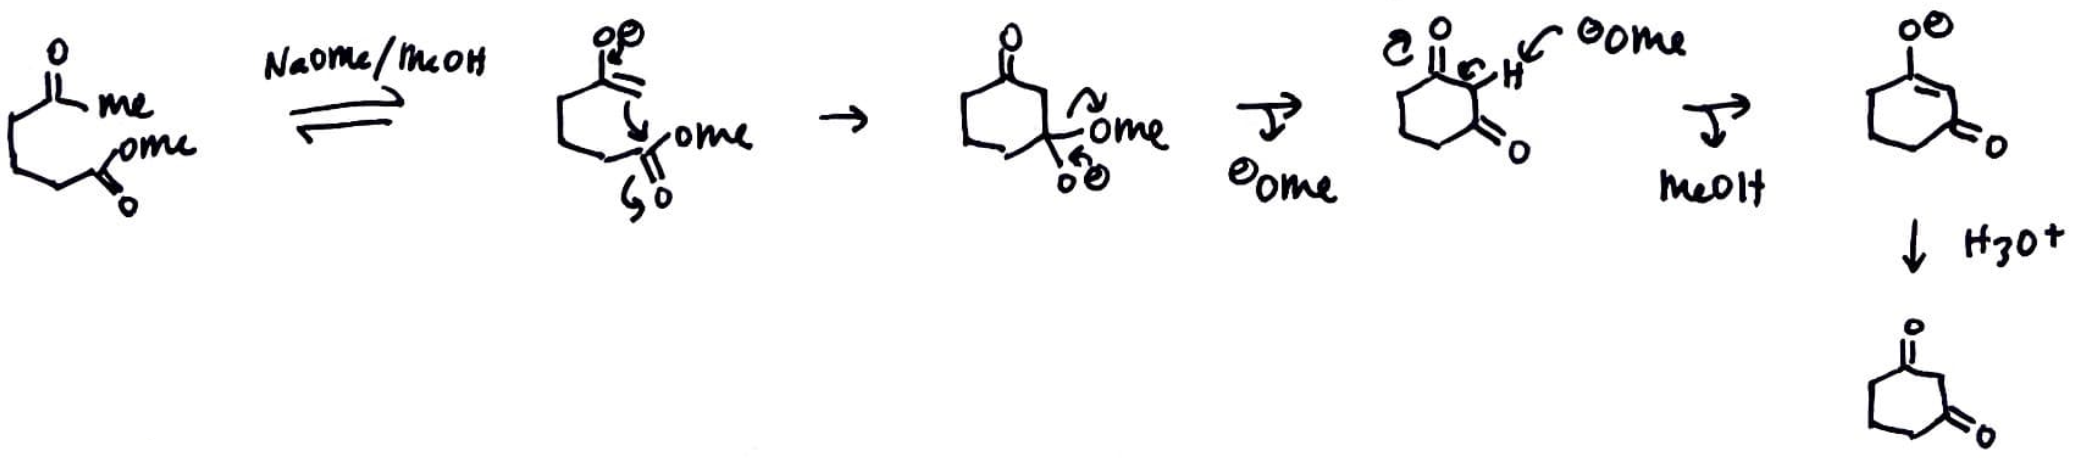
\includegraphics[width=0.95\linewidth]{DieckmannMech.png}
        \caption{Dieckmann condensation mechanism.}
        \label{fig:DieckmannMech}
    \end{figure}
    \begin{itemize}
        \item Making 1,3-diones is a topic that will probably be on the exam!! Prof. Buchwald likes these questions.
    \end{itemize}
    \item Crossed or mixed Claisen condensations.
    \begin{figure}[h!]
        \centering
        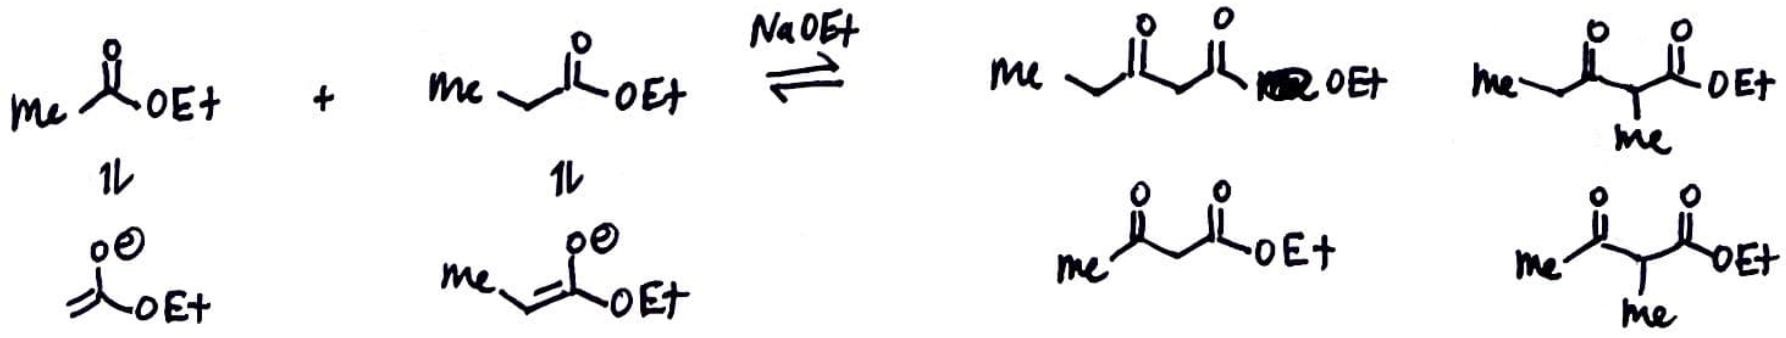
\includegraphics[width=0.8\linewidth]{mixedClaisen.png}
        \caption{Mixed Claisen condensation product distribution.}
        \label{fig:mixedClaisen}
    \end{figure}
    \pagebreak
    \begin{itemize}
        \item Claisen reactions don't have to be dimerizations!
        \item If we mix two esters, we will not get the coupled product selectively.
        \begin{itemize}
            \item Instead, we will get a mixture, and \emph{we do not like mixtures}.
        \end{itemize}
        \item Recall that \ce{NaOEt} only yields a small amount of enolate, so once it's formed, it can react with either compound.
    \end{itemize}
    \item Effective mixed Claisen.
    \begin{figure}[h!]
        \centering
        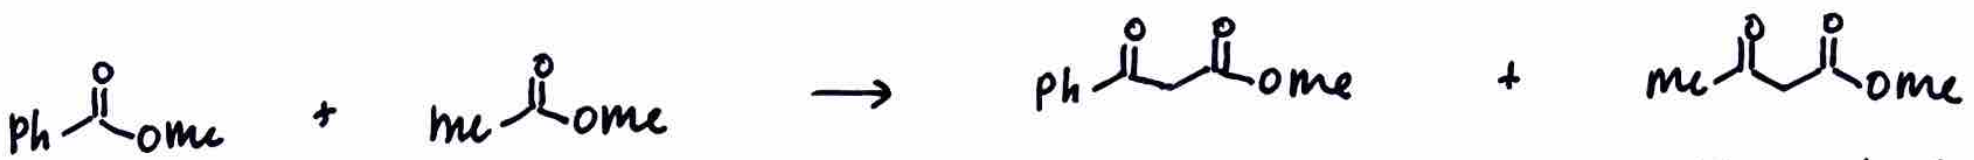
\includegraphics[width=0.85\linewidth]{crossClaisenOne.png}
        \caption{Cross-Claisen condensation with only one enolizable species.}
        \label{fig:crossClaisenOne}
    \end{figure}
    \begin{itemize}
        \item Analogously to Figure \ref{fig:crossAldolOne}, we can use a mixture containing only one enolizable position.
        \item One side product we'd see is the dimerization product of the enolizable species.
        \begin{itemize}
            \item If we were desperate to make this compound, though, we could do this and then purify out just the heterocoupled product.
        \end{itemize}
        \item Thus, this is still inelegant.
    \end{itemize}
    \item Solution \#1 to mixed Claisens.
    \begin{figure}[h!]
        \centering
        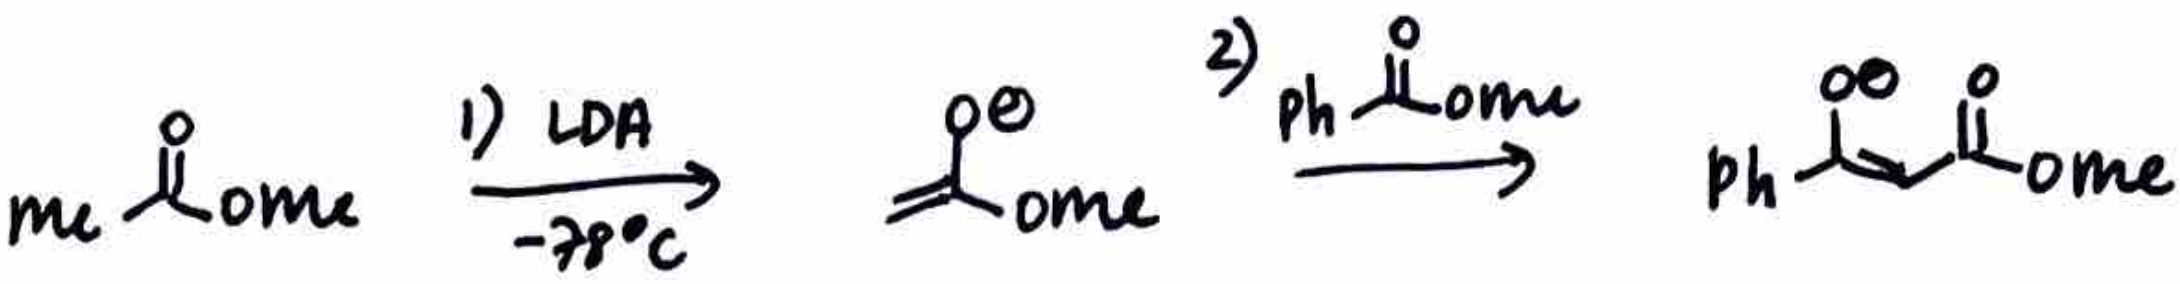
\includegraphics[width=0.65\linewidth]{crossClaisenModern.png}
        \caption{Modern cross-Claisen condensation.}
        \label{fig:crossClaisenModern}
    \end{figure}
    \begin{itemize}
        \item Analogously to Figure \ref{fig:crossAldolModern}, use LDA!
        \item One-pot, two-step process: To a container of your first ester in THF at $-\SI{78}{\celsius}$, add LDA. Then add your other ester.
    \end{itemize}
    \item Solution \#2 to mixed Claisens.
    \begin{figure}[h!]
        \centering
        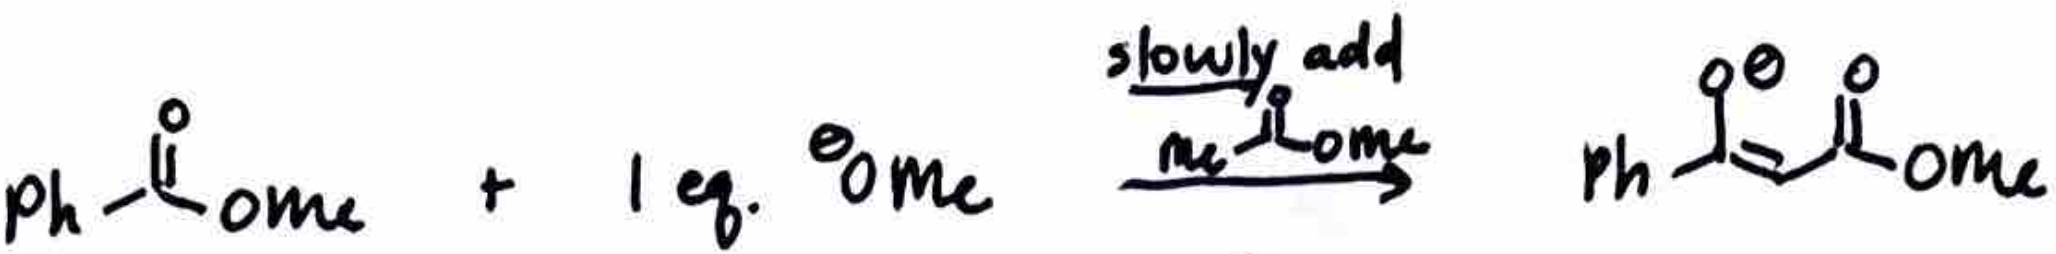
\includegraphics[width=0.55\linewidth]{crossClaisenDrop.png}
        \caption{Dropwise cross-Claisen condensation.}
        \label{fig:crossClaisenDrop}
    \end{figure}
    \begin{itemize}
        \item Mix your nonenolizable ester and base. Then add your other ester slowly/dropwise.
        \item This makes it so that as soon as a molecule of your enolizable ester forms the enolate, it is surrounded by many more molecules of the nonenolizable ester and thus is more likely to react with one of them!
    \end{itemize}
    \item Reactions between ketones and esters are usually clean.
    \begin{figure}[h!]
        \centering
        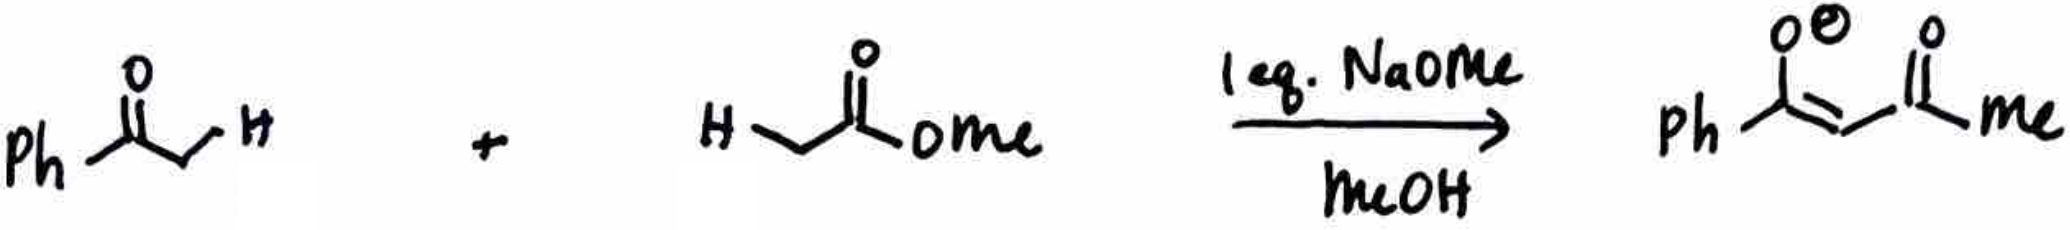
\includegraphics[width=0.65\linewidth]{ketoneEster.png}
        \caption{Ketone-ester condensation.}
        \label{fig:ketoneEster}
    \end{figure}
    \begin{itemize}
        \item Here, we take advantage of the difference in $\pKa$'s.
        \begin{itemize}
            \item Essentially, we will form \num{e6} times more ketone enolate than ester enolate because $\pKa\approx 19$ at the $\alpha$-position of a ketone, and $\pKa\approx 25$ at the $\alpha$-position of an ester.
        \end{itemize}
        \item Takeaway: $\Delta\pKa$'s control the selectivity.
        \item However, there is one complication.
        \begin{itemize}
            \item Because ketones are more electrophilic than esters, the (non-dehydrogenated) aldol will form in solution more readily than the Claisen condensation product.
            \item However, the aldol product forms reversibly, and the Claisen one does not!
            \item Thus, the quick reversible equilibrium to the aldol product gives way to a slow, steady, and irreversible conversion to the Claisen condensation product, forming it exclusively in the end.
        \end{itemize}
    \end{itemize}
    \item This concludes our discussion of Claisen condensations.
    \item We now move onto Topic F: Michael additions.
    \begin{itemize}
        \item These are also known as 1,4-additions.
    \end{itemize}
    \item General form.
    \begin{figure}[h!]
        \centering
        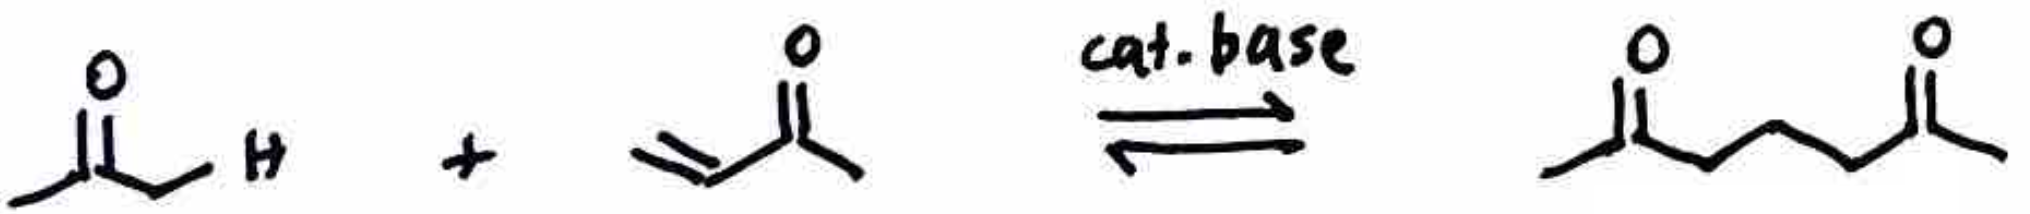
\includegraphics[width=0.5\linewidth]{michael.png}
        \caption{Michael addition.}
        \label{fig:michael}
    \end{figure}
    \begin{itemize}
        \item We run these reactions with catalytic base.
        \item In retrosynthesis, look for 1,5-dicarbonyls! This is a big clue that Michael addition was used.
        \item The left compound (the enolizable ketone) is called a \textbf{Michael donor}.
        \begin{itemize}
            \item It is nucleophilic.
            \item Examples: The enolates of esters, ketones, and 1,3-dicarbonyl compounds.
        \end{itemize}
        \item The right compound (the $\alpha,\beta$-unsaturated ketone) is called a \textbf{Michael acceptor}.
        \begin{itemize}
            \item It is electrophilic.
            \item Examples: $\alpha,\beta$-unsaturated acyl \ce{X} groups, where $\ce{X}=\ce{H},\text{alkyl},\text{aryl},\ce{OR},\ce{NR2}$, etc. $\alpha,\beta$-unsaturated nitriles and nitro-compounds work, too.
        \end{itemize}
    \end{itemize}
    \item Why do we get nucleophilic attack at the $\alpha,\beta$-unsaturated ketone's $\beta$-carbon?
    \begin{figure}[h!]
        \centering
        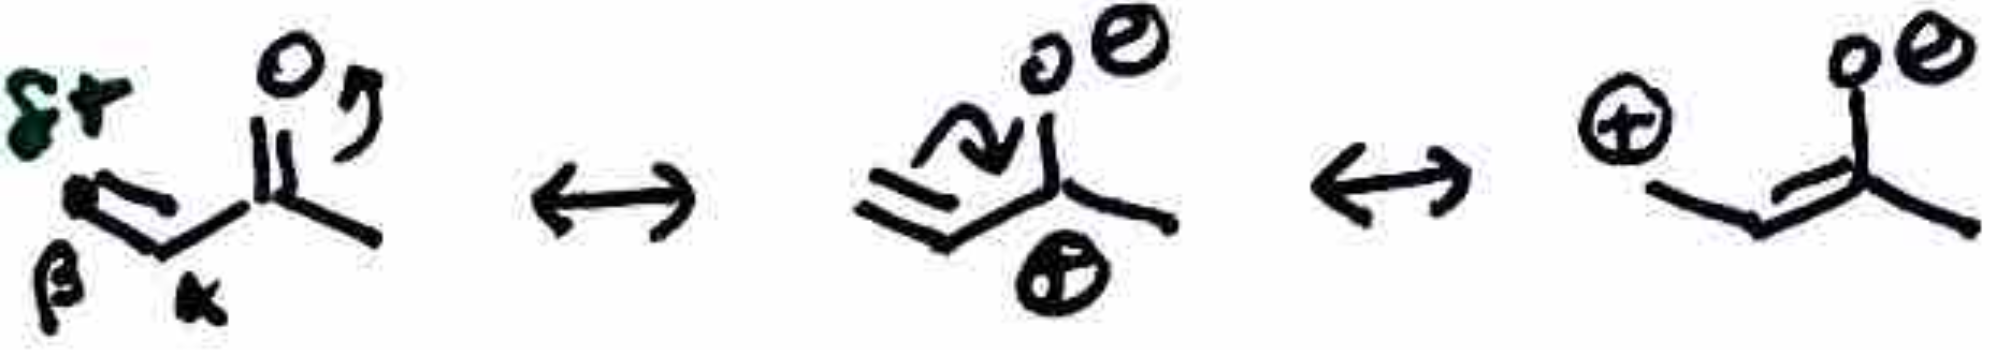
\includegraphics[width=0.4\linewidth]{enoneForm.png}
        \caption{Resonance forms of an $\alpha,\beta$-unsaturated ketone.}
        \label{fig:enoneForm}
    \end{figure}
    \begin{itemize}
        \item Because of resonance, that $\beta$-carbon has a $\delta^+$ partial charge on it!
    \end{itemize}
    \item Michael addition mechanism.
    \begin{figure}[h!]
        \centering
        \includegraphics[width=0.9\linewidth]{michaelMech.png}
        \caption{Michael addition mechanism.}
        \label{fig:michaelMech}
    \end{figure}
    \begin{itemize}
        \item The Michael donor gets converted to its enolate form, which then attacks the Michael acceptor.
    \end{itemize}
    \pagebreak
    \item Example Michael addition.
    \begin{figure}[h!]
        \centering
        \includegraphics[width=0.5\linewidth]{michaelIntra.png}
        \caption{Intramolecular Michael addition.}
        \label{fig:michaelIntra}
    \end{figure}
    \begin{itemize}
        \item This type of reaction leads into another important reaction!
    \end{itemize}
    \item The Robinson annulation.
    \begin{figure}[h!]
        \centering
        \includegraphics[width=0.55\linewidth]{robinson.png}
        \caption{Robinson annulation.}
        \label{fig:robinson}
    \end{figure}
    \begin{itemize}
        \item This reaction is a Michael addition, followed by an aldol condensation, followed by a dehydration.
        \item A historically important reaction that is still used today to synthesize pharmaceuticals at scale.
    \end{itemize}
    \item 1,4-additions are a broader class of reactions than just Michael additions.
    \begin{itemize}
        \item Recall Figure \ref{fig:AddClCu}: Gilman reagents can do a kind of 1,4-addition, too!
        \item Note that we can synthesize a broader class of Gilman reagents called \textbf{cuprates} by combining 2 equivalents of an alkyllithium reagent \ce{RLi} with \ce{CuI}; these \ce{R2CuLi} reagents will then add \ce{R} instead of \ce{Me}!
    \end{itemize}
    \item If we have an $\alpha,\beta$-unsaturated ketone, a Grignard or alkyllithium reagent could be used to do 1,2-addition to the ketone.
    \begin{figure}[h!]
        \centering
        \footnotesize
        \schemestart
            \chemfig{*6(----(=O)-=)}
            \arrow{->[\ce{MeMgBr}][or \ce{MeLi}]}[,1.4]
            \chemfig{*6(----(-[:70]Me)(-[:110]\charge{135=$\ominus$}{O})-=)}
        \schemestop
        \caption{1,2-addition with Grignards and alkyllithium reagents.}
        \label{fig:12add}
    \end{figure}
    \begin{itemize}
        \item This is called 1,2-addition because we add a metal (\ce{Mg} or \ce{Li}) to the 1-atom (the oxygen), and an \ce{R} group to the 2-atom (the carbon).
    \end{itemize}
    \item If we have an $\alpha,\beta$-unsaturated ketone, a Gilman reagent can do 1,4-addition to the entire enone system!
    \begin{figure}[h!]
        \centering
        \includegraphics[width=0.35\linewidth]{14add.png}
        \caption{1,4-addition with the Gilman reagent.}
        \label{fig:14add}
    \end{figure}
    \begin{itemize}
        \item This is called 1,4-addition because we add a metal (\ce{Cu}) to the 1-atom (the oxygen), and an \ce{R} group to the 4-atom (the $\beta$-position).
    \end{itemize}
    \item 1,4-addition also gives us an enolate, and an enolate is a terrible thing to waste.
    \begin{itemize}
        \item We can work this up directly to get rid of it, \emph{or} we can use it.
        \item For instance, we could trap it as a silyl enol ether (as in Figure \ref{fig:enolateTMS}).
        \begin{itemize}
            \item Recall that we could then regenerate the enolate later with \ce{MeLi}.
        \end{itemize}
    \end{itemize}
\end{itemize}




\end{document}